\section{Comparing Cislunar Departure Families}
In this investigation, unstable periodic orbits in the Earth-Moon CR3BP are considered as potential
departure orbits for deep space transfers. Several orbit families with unstable members are
introduced in Section 3.2 and from these families, unstable orbits between Jacobi constants of
$2.98$ and $3.13$ are analyzed to determine their feasibility for these transfers. This range was
chosen since the upper energy bound of $2.98$ is slightly above the energy level of the $L_{4}$ and
$L_{5}$ Lagrange points, while the lower bound includes a large number of the unstable libration
orbits\cite{Zimovan:2017}. Note that not all of the included families have unstable orbits at these
energy levels. Additionally, in some instances, even though the orbits existed, their stability,
energy, or location prevented their unstable invariant manifolds from interfacing with the stable
manifolds of the staging orbit or departing the system promptly. Several other periodic orbit
families were also investigated, including $L_{4}$ and $L_{5}$ long-period orbits and some unstable
resonant orbit families. However, invariant manifolds from orbits in these families also took too
long to depart the system for this investigation.

For the feasible departure orbits, the cost function described previously is used to determine the
most desirable end-to-end transfers in the orbit's tradespace, and then the average total
maneuver $\Delta v$ and TOF costs are compared between the various departure orbits in this
investigation. While no one orbit or family of orbits provides the best transfers across the
different energy levels, some trends can be extracted from the results to inform cislunar departure
orbit selection for these types of missions.

\subsection{Contributing Factors for Lower Total Maneuver Costs}
Of the two maneuvers, or three if using a staging orbit, in the end-to-end transfer, the largest is
the final burn that includes the inclination change between the Sun-Earth and Sun-Mars planes.
Plane change maneuvers are most efficient at a conic orbit's apoapsis, so this maneuver $\Delta v$
is lower when the MMAT bridge conic true anomaly at the intersection of the conic sections,
$\theta_{b_{int}}$, is near $\ang{180}$. This also requires that the departure and bridge conics
are oriented such that their apoapses are near the line of nodes since the inclination change must
occur at either the ascending or descending node. The conic intersection location is a function of
the relative orientations of the departure and arrival conics, which are dependent on the phasing
of the departure from and arrival at the two planetary systems. 

As mentioned, the cost function identifies the transfers with the lowest cost, considering both the
maneuver cost and TOF. Therefore, among the ten best transfers in a tradespace, there will be ones
with lower total $\Delta v$ and and ones with a lower TOF.
\cref{fig:stagedMinDvEM}-\cref{fig:stagedMinDvMMAT} show an example staging orbit low-$\Delta v$
case departing from a northern $L_{1}$ halo orbit, with a total maneuver cost of $4.781$ km/s and
TOF of $5.21$ years. Likewise, \cref{fig:directMinDvE} and \cref{fig:directMinDvMMAT} show a direct
example departing from an $L_{1}$ Lyapunov orbit, with a total maneuver cost of $4.55$ km/s and TOF
of $4.49$ years. In both MMAT figures, \cref{fig:stagedMinDvMMAT} and \cref{fig:directMinDvMMAT},
the two maneuvers occur approximately $\ang{180}$ apart from each other, and since the first burn
is constrained to be at the periapsis of the bridge conic, the second burn is near apoapsis. Note
that in the transfer example with direct departure, the manifold arc chosen departs on the $L_{2}$
side of the Sun-Earth system. This is consistent for lower-$\Delta v$ direct transfers across all
the departure orbits analyzed in this investigation.

\begin{figure}[!htb]
    \centering
    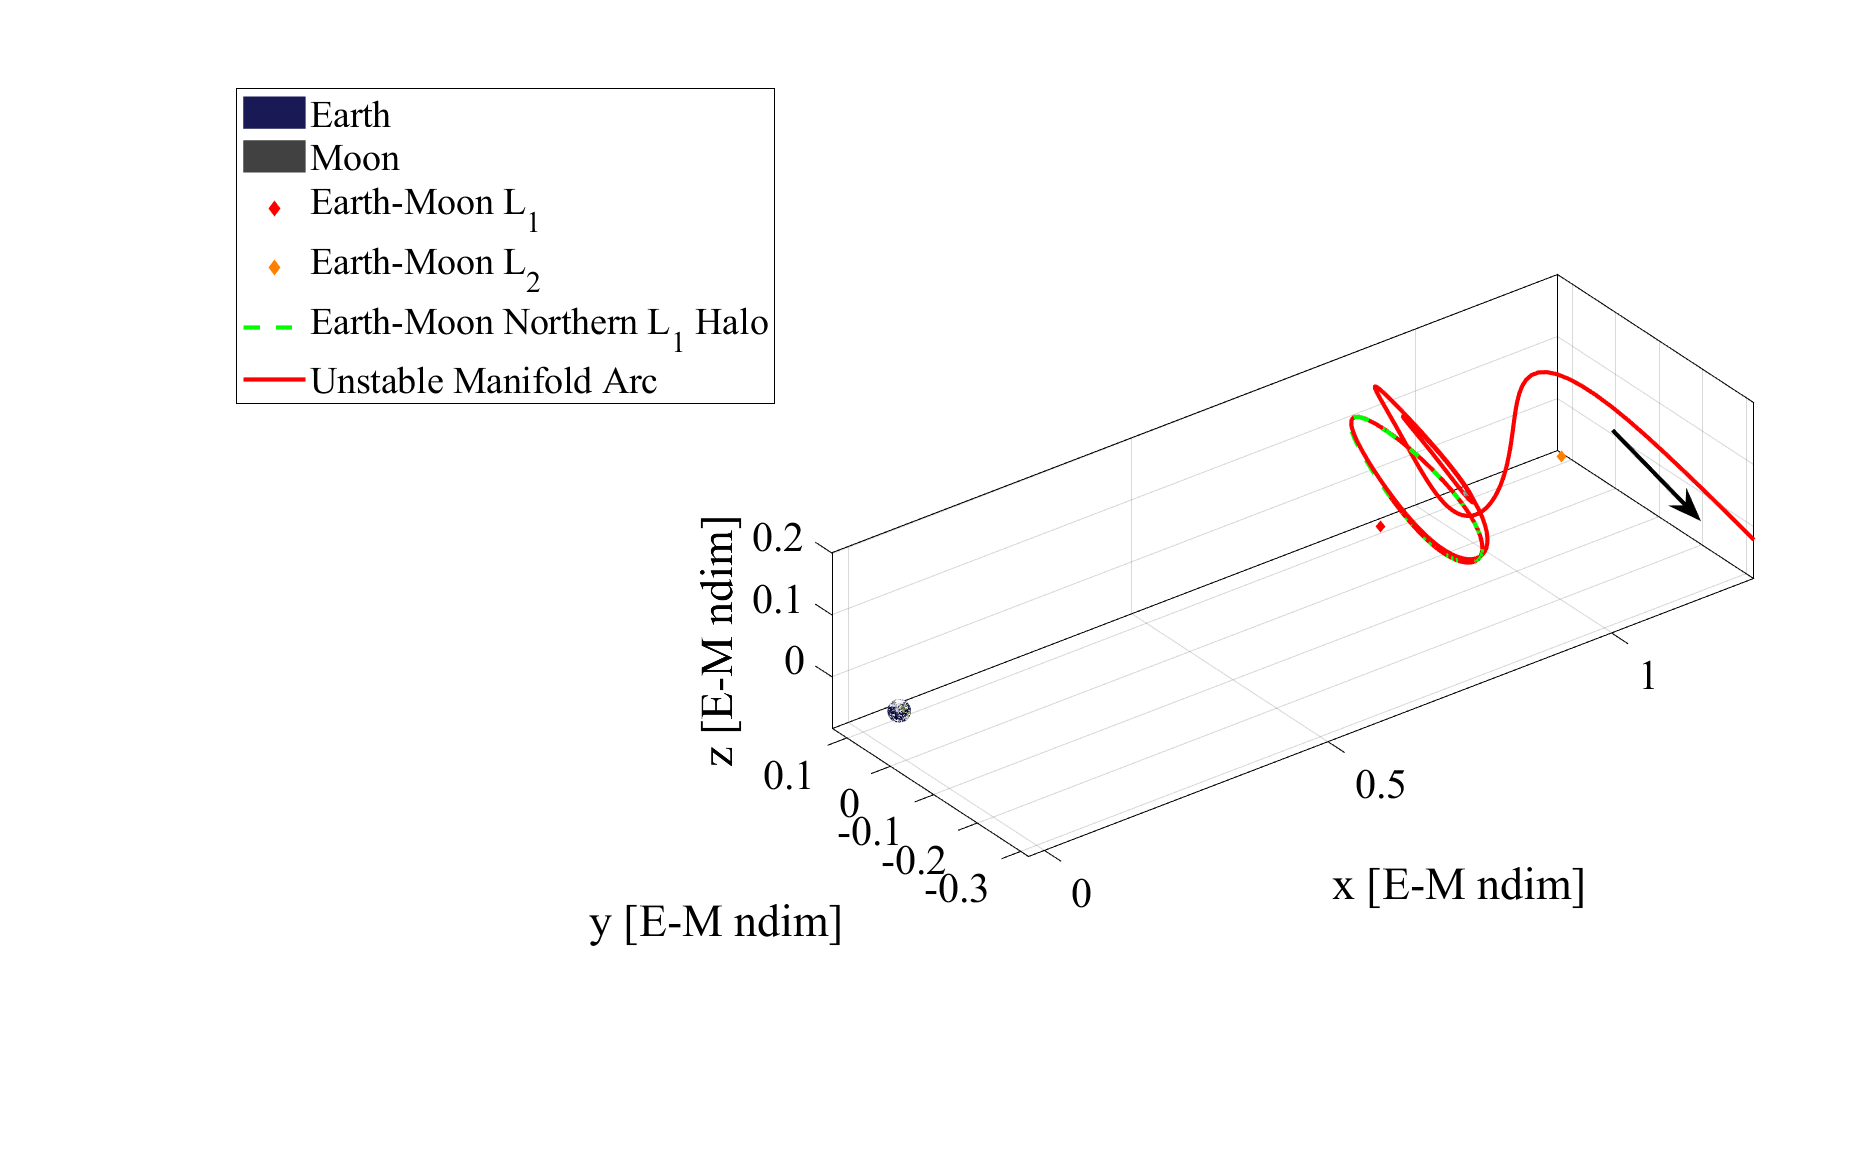
\includegraphics[width=0.9\textwidth]{figures/StagedMinDvEM.pdf}
    \caption{Northern $L_{1}$ halo orbit ($JC=3.03$) departure manifold arc in the Earth-Moon barycentric rotating frame for a low-$\Delta v$ case.}
    \label{fig:stagedMinDvEM}
\end{figure}

\begin{figure}[!htb]
    \centering
    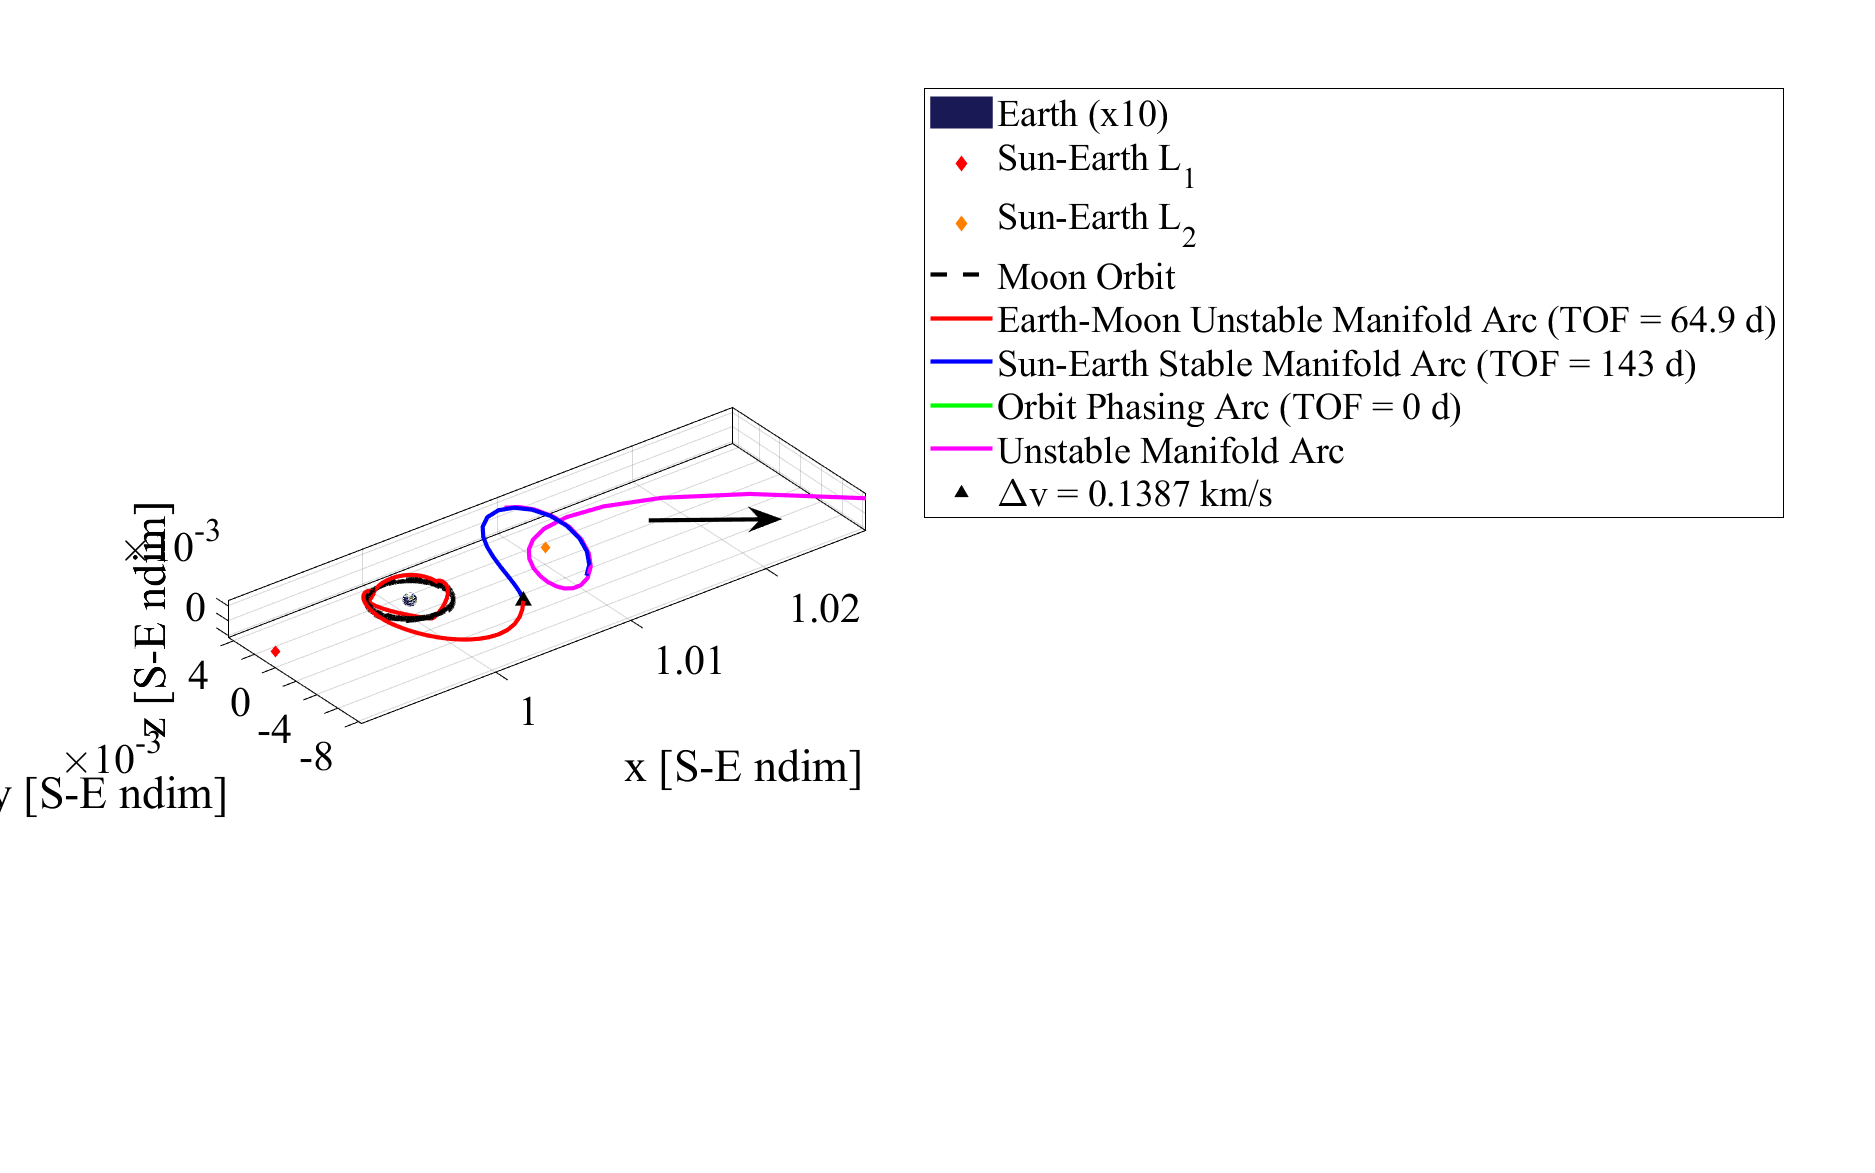
\includegraphics[width=0.9\textwidth]{figures/StagedMinDvSE.pdf}
    \caption{Departure CR3BP arc with northern $L_{2}$ halo staging orbit ($JC=3.000808$) in the Sun-Earth barycentric rotating frame for a low-$\Delta v$ case.}
    \label{fig:stagedMinDvSE}
\end{figure}

\begin{figure}[!htb]
    \centering
    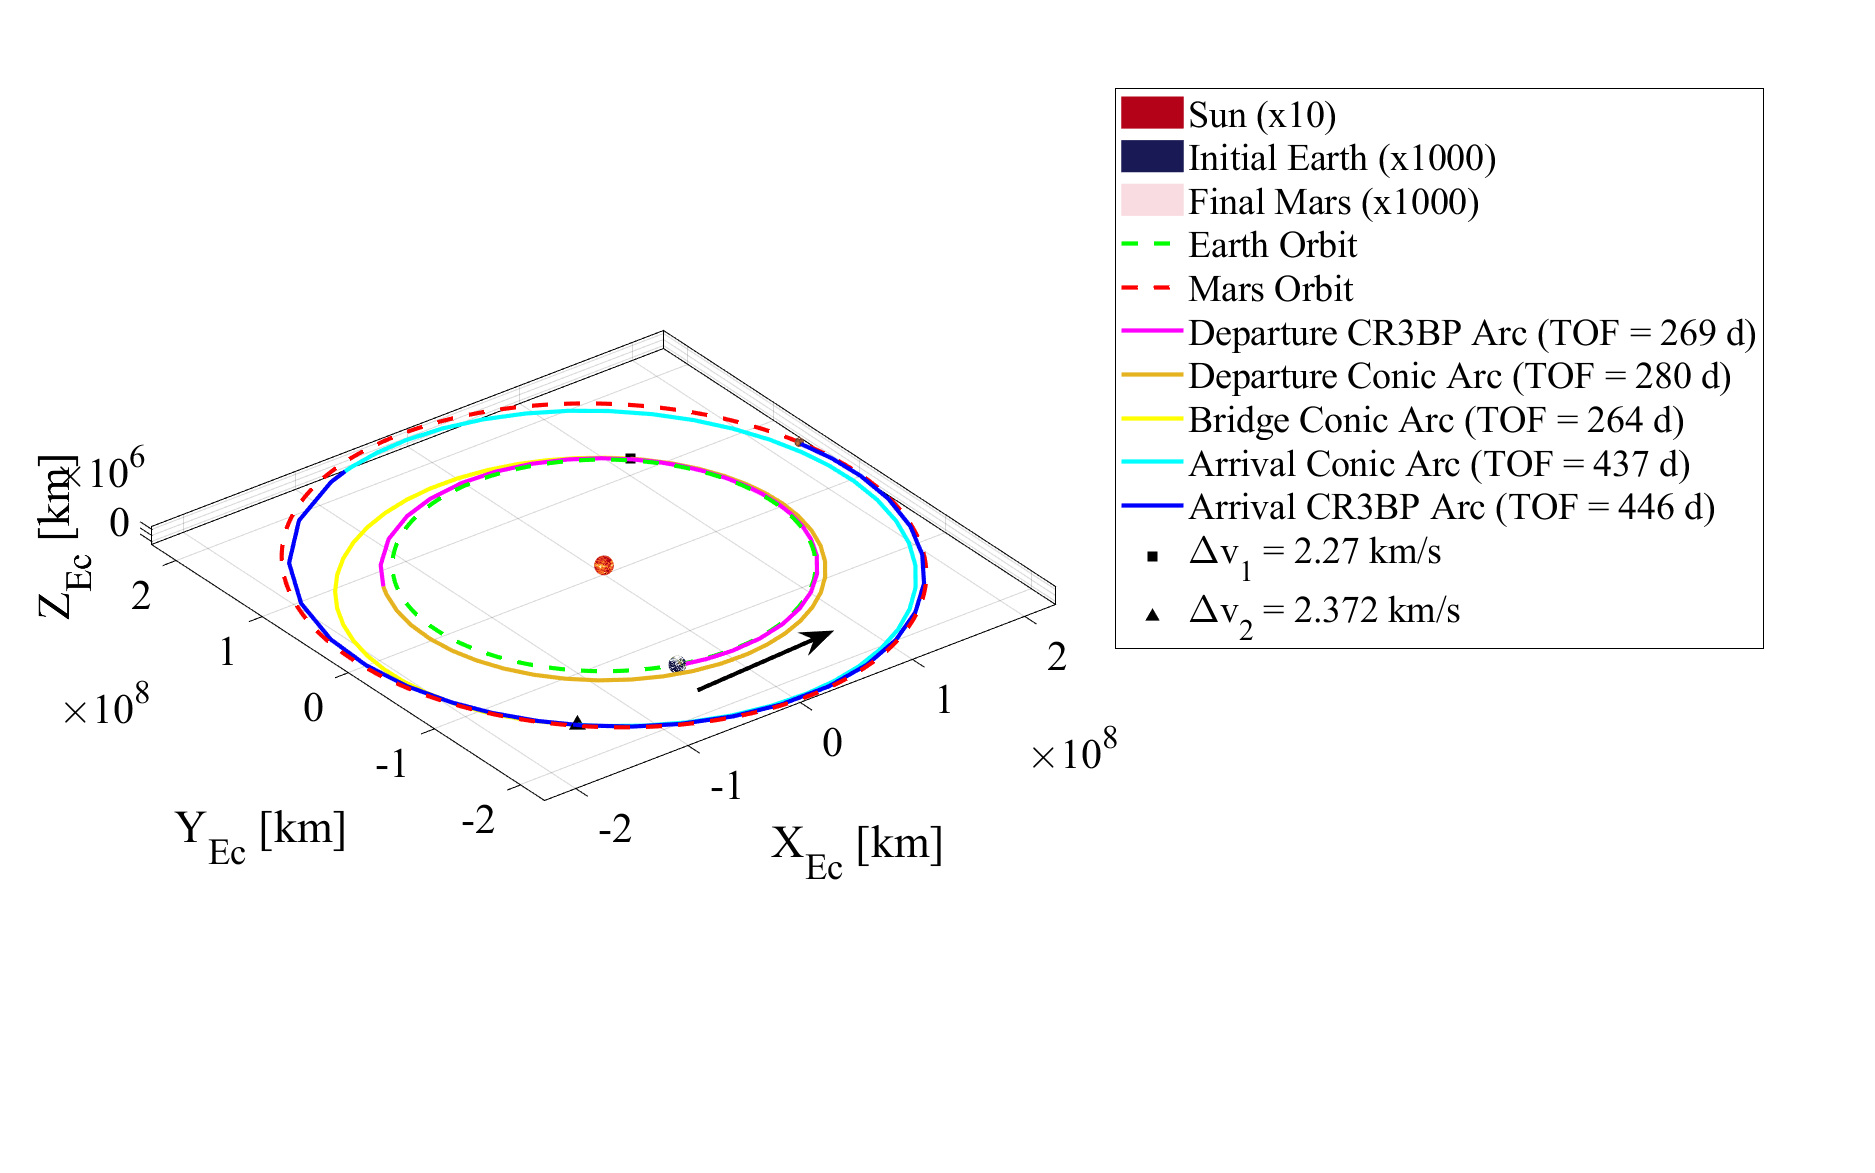
\includegraphics[width=0.9\textwidth]{figures/StagedMinDvMMAT.pdf}
    \caption{MMAT in the Sun-centered Ecliptic J2000 frame for a staging orbit low-$\Delta v$ case.}
    \label{fig:stagedMinDvMMAT}
\end{figure}

\begin{figure}[!htb]
    \begin{subfigure}[h]{0.495\linewidth}
        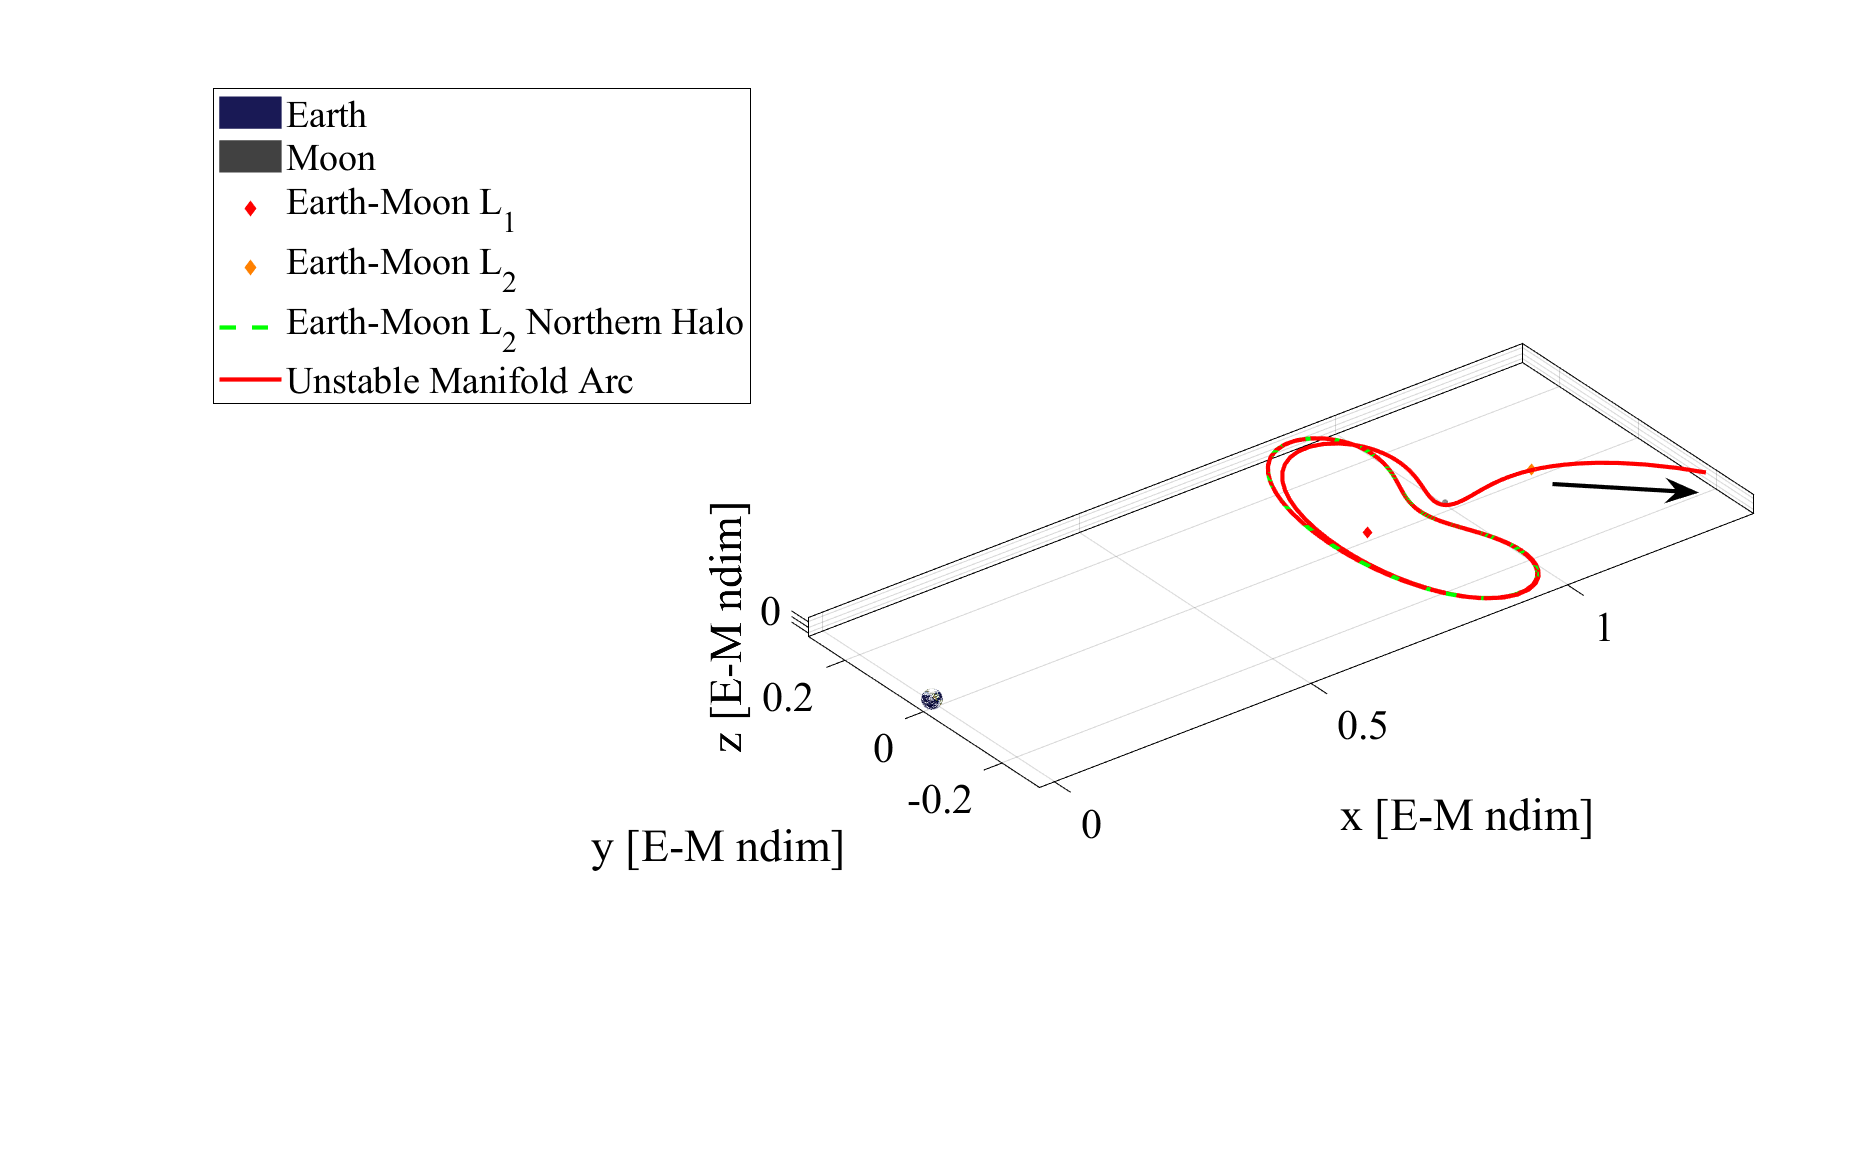
\includegraphics[width=\textwidth]{figures/DirectMinDvEM.pdf}
        \caption{Earth-Moon barycentric rotating frame.}
    \end{subfigure}
    \hfill
    \begin{subfigure}[h]{0.495\linewidth}
        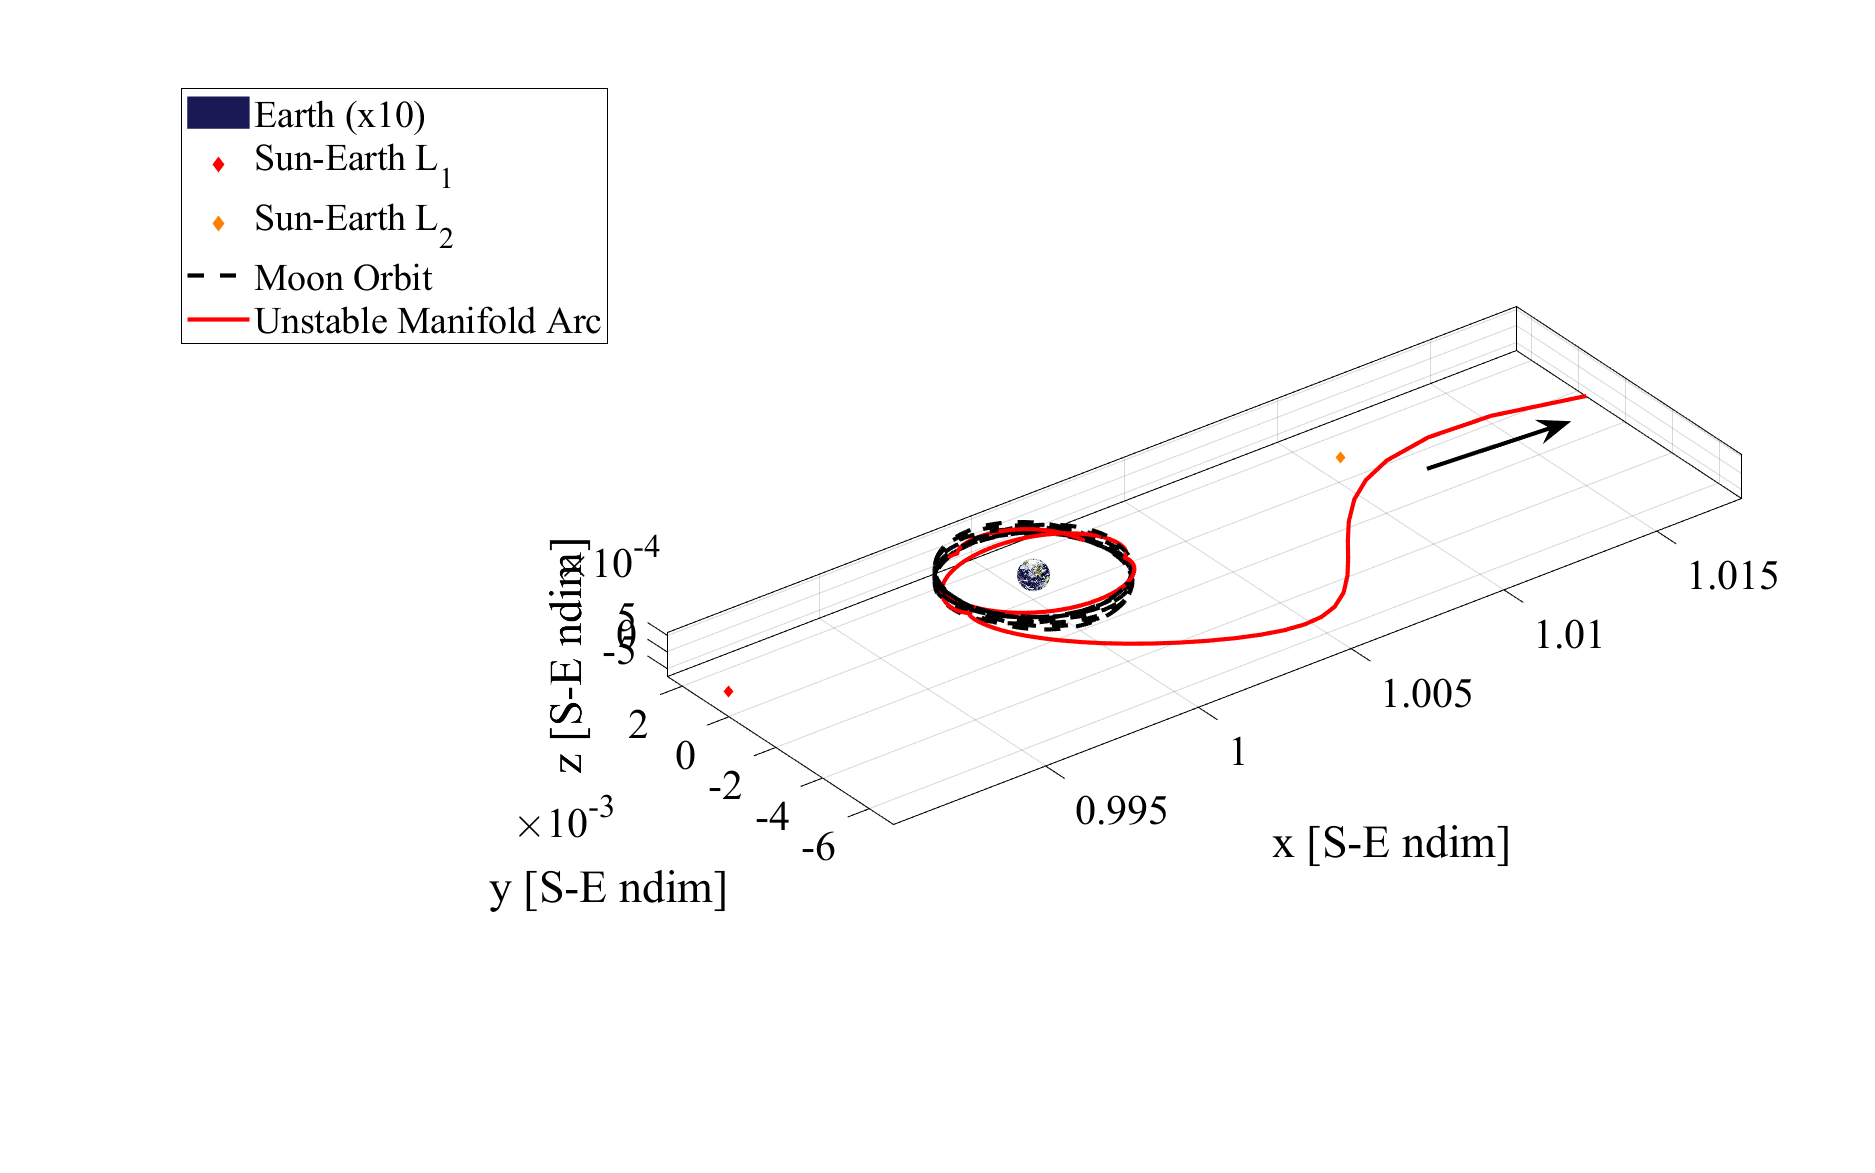
\includegraphics[width=\textwidth]{figures/DirectMinDvSE.pdf}
        \caption{Sun-Earth barycentric rotating frame.}
    \end{subfigure}
    \caption{$L_{1}$ Lyapunov orbit ($JC=3.0$) departure CR3BP arc for a low-$\Delta v$ case.}
    \label{fig:directMinDvE}
\end{figure}

\begin{figure}[!htb]
    \centering
    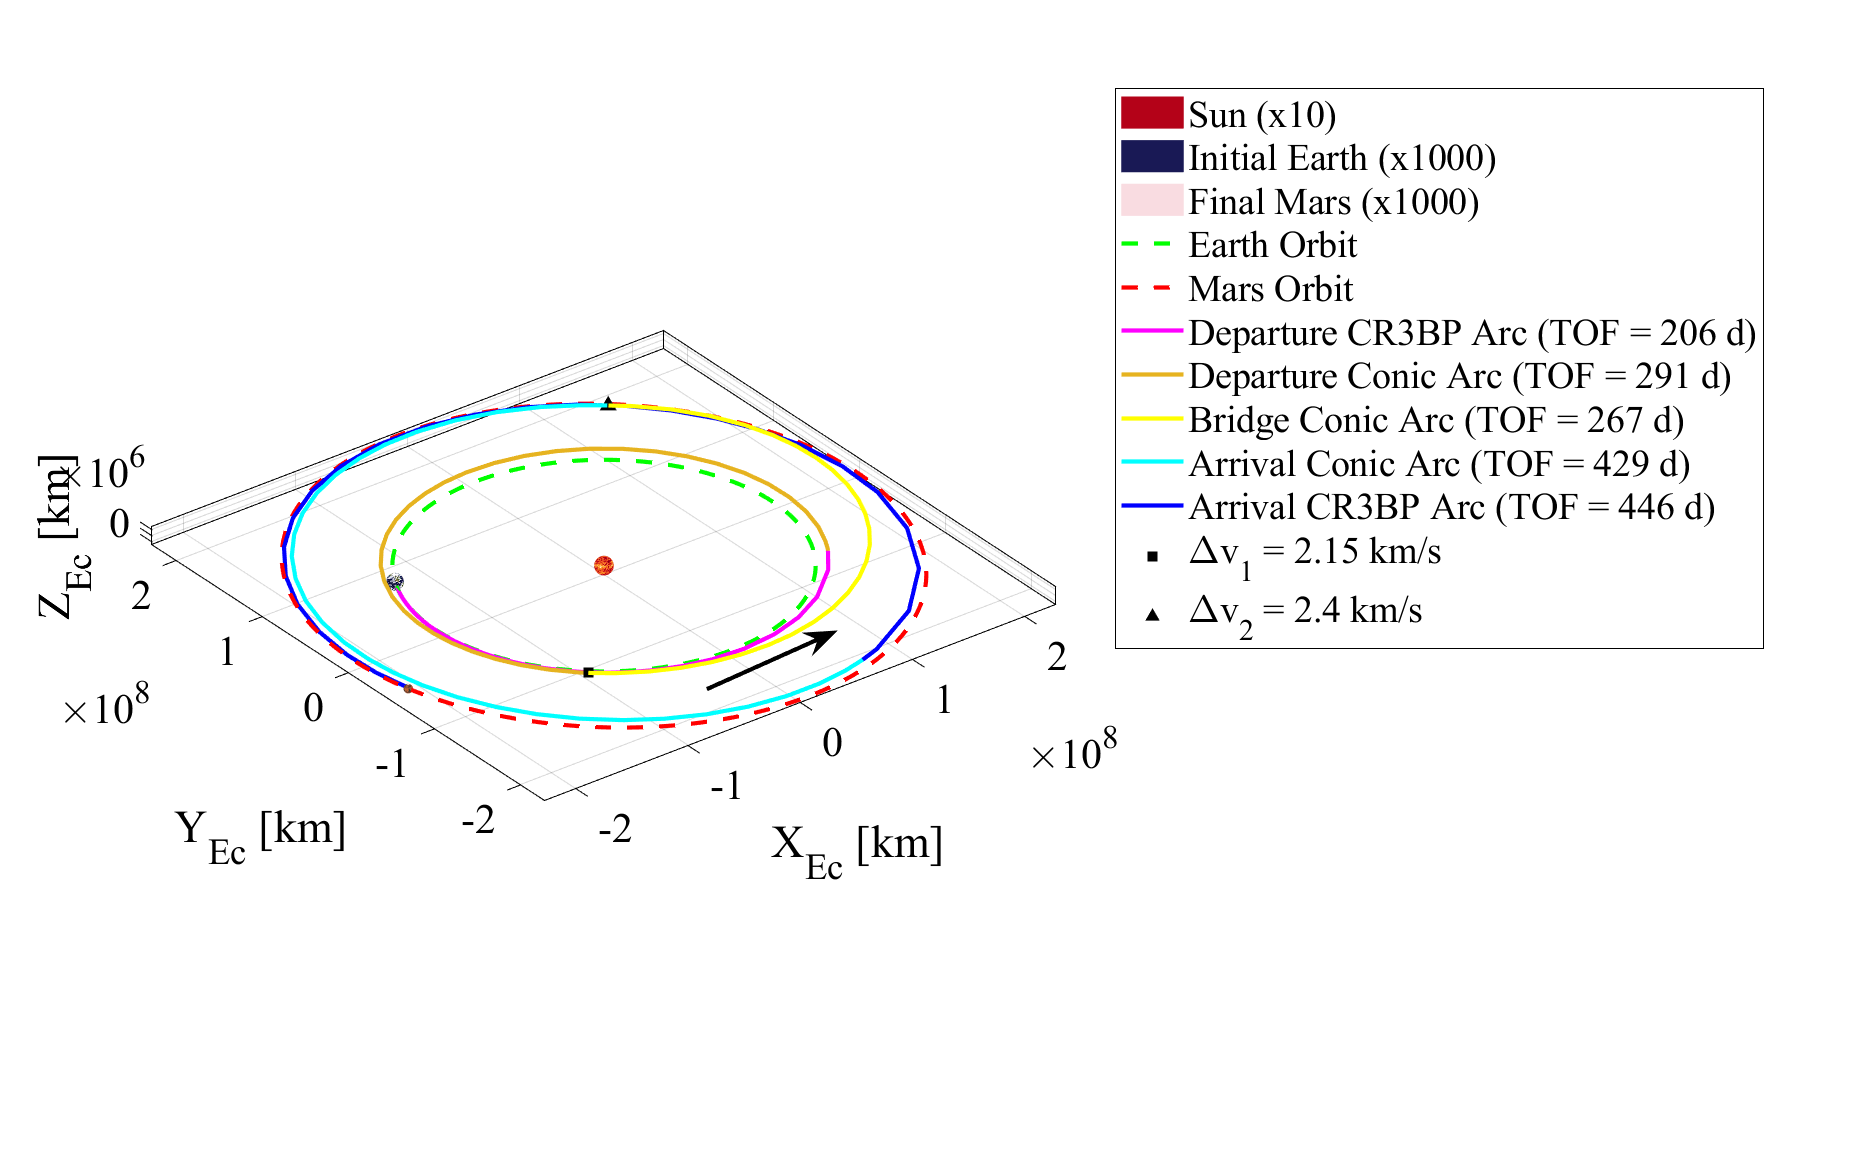
\includegraphics[width=0.9\textwidth]{figures/DirectMinDvMMAT.pdf}
    \caption{MMAT in the Sun-centered Ecliptic J2000 frame for a direct low-$\Delta v$ case.}
    \label{fig:directMinDvMMAT}
\end{figure}

Beyond the relative orientation between the two MMAT maneuvers, the energy gap between the
departure and arrival arcs (and thereby the Sun-Earth and Sun-Mars CR3BP arcs, respectively) also
contributes to the total $\Delta v$. A larger difference requires a higher-cost maneuver to change
the Keplerian conic energy from the departure arc to that of the arrival arc; these energies are
determined by the manifold arcs chosen and the phasing of the two planetary systems. This
highlights the importance of families of transfer solutions. Since several interdependent factors
affect the total maneuver cost, it is necessary to search through the results across families of
solutions to find low-$\Delta v$ solution basins.

\subsection{Contributing Factors for Lower Total Times-of-Flight}
While $\Delta v$ is primarily dependent on the final MMAT maneuver location, the biggest factor
affecting time-of-flight is the relative orientation of the departure and arrival conic arcs. Since
these are dependent on their respective CR3BP manifold arcs, the phasing of the two planetary
systems at departure and arrival largely dictate the total transfer TOF. As mentioned, the first
MMAT maneuver occurs at the periapsis of the departure conic arc. Therefore, to minimize the time
along the departure conic arc, its periapsis should be just after the Sun-Earth CR3BP SoI
intersection. Similarly, although the true anomaly of the intersection between the bridge and
arrival arcs can vary, it should be just before the Sun-Mars CR3BP SoI intersection true anomaly to
minimize the time along the arrival conic arc.

As it turns out, the time along the arrival conic arc is easier to decrease than that of the
departure conic arc. \cref{fig:stagedMinTOFEM}-\cref{fig:stagedMinTOFMMAT} show a low-TOF case from
the best staging orbit transfers of a northern $L_{2}$ halo orbit, with a total maneuver cost of
$5.582$ km/s and TOF of $4.25$ years. Departing from the same $JC=3.13$ northern $L_{1}$ halo
orbit, the transfer shown in \cref{fig:directMinTOFE} and \cref{fig:directMinTOFMMAT} has a total
maneuver cost of $5.624$ km/s and TOF of $3.19$ years. In \cref{fig:stagedMinTOFMMAT} and
\cref{fig:directMinTOFMMAT}, the TOF of the arrival conic arc is minimal compared to the other legs
of the transfer, while the departure conic arc TOF remains about as large as the other solutions.
In the Sun-Earth rotating frame representation of the direct departure transfer,
\cref{fig:directMinTOFE}(b), the manifold arc again departs on the $L_{2}$ side of the Sun-Earth
system. This is because the best solutions chosen with the cost function tend to be closer to the
minimum-$\Delta v$ cases instead of the minimum-TOF transfers. So the lowest-TOF transfer among the
best solutions is still closer to a minimum-$\Delta v$ case. For the truly minimum-TOF transfers,
with maneuver costs much higher than the modified Hohmann transfer baseline, the unstable manifold
arcs depart on the Sun-Earth $L_{1}$ side.

\begin{figure}[!htb]
    \centering
    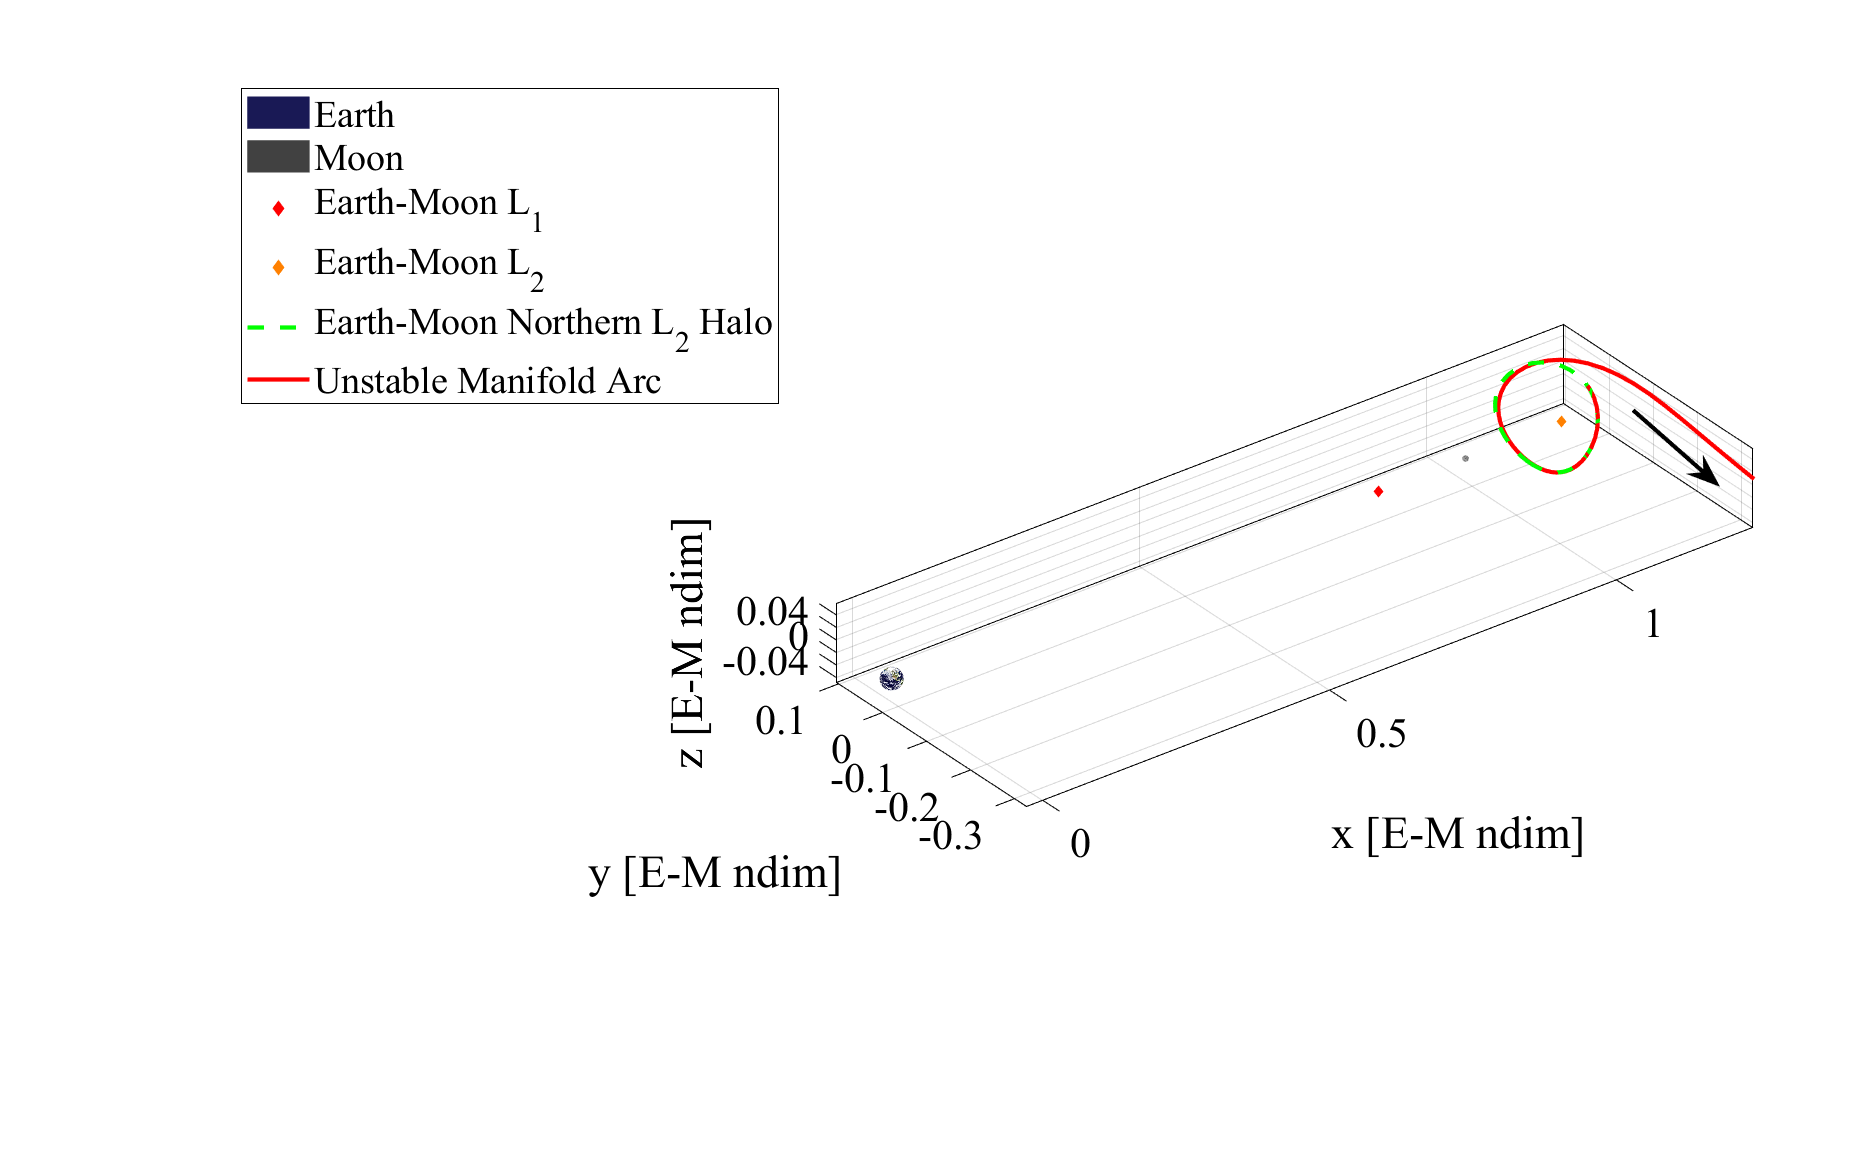
\includegraphics[width=0.9\textwidth]{figures/StagedMinTOFEM.pdf}
    \caption{Northern $L_{2}$ halo orbit ($JC=3.13$) departure manifold arc in the Earth-Moon barycentric rotating frame for a low-TOF case.}
    \label{fig:stagedMinTOFEM}
\end{figure}

\begin{figure}[!htb]
    \centering
    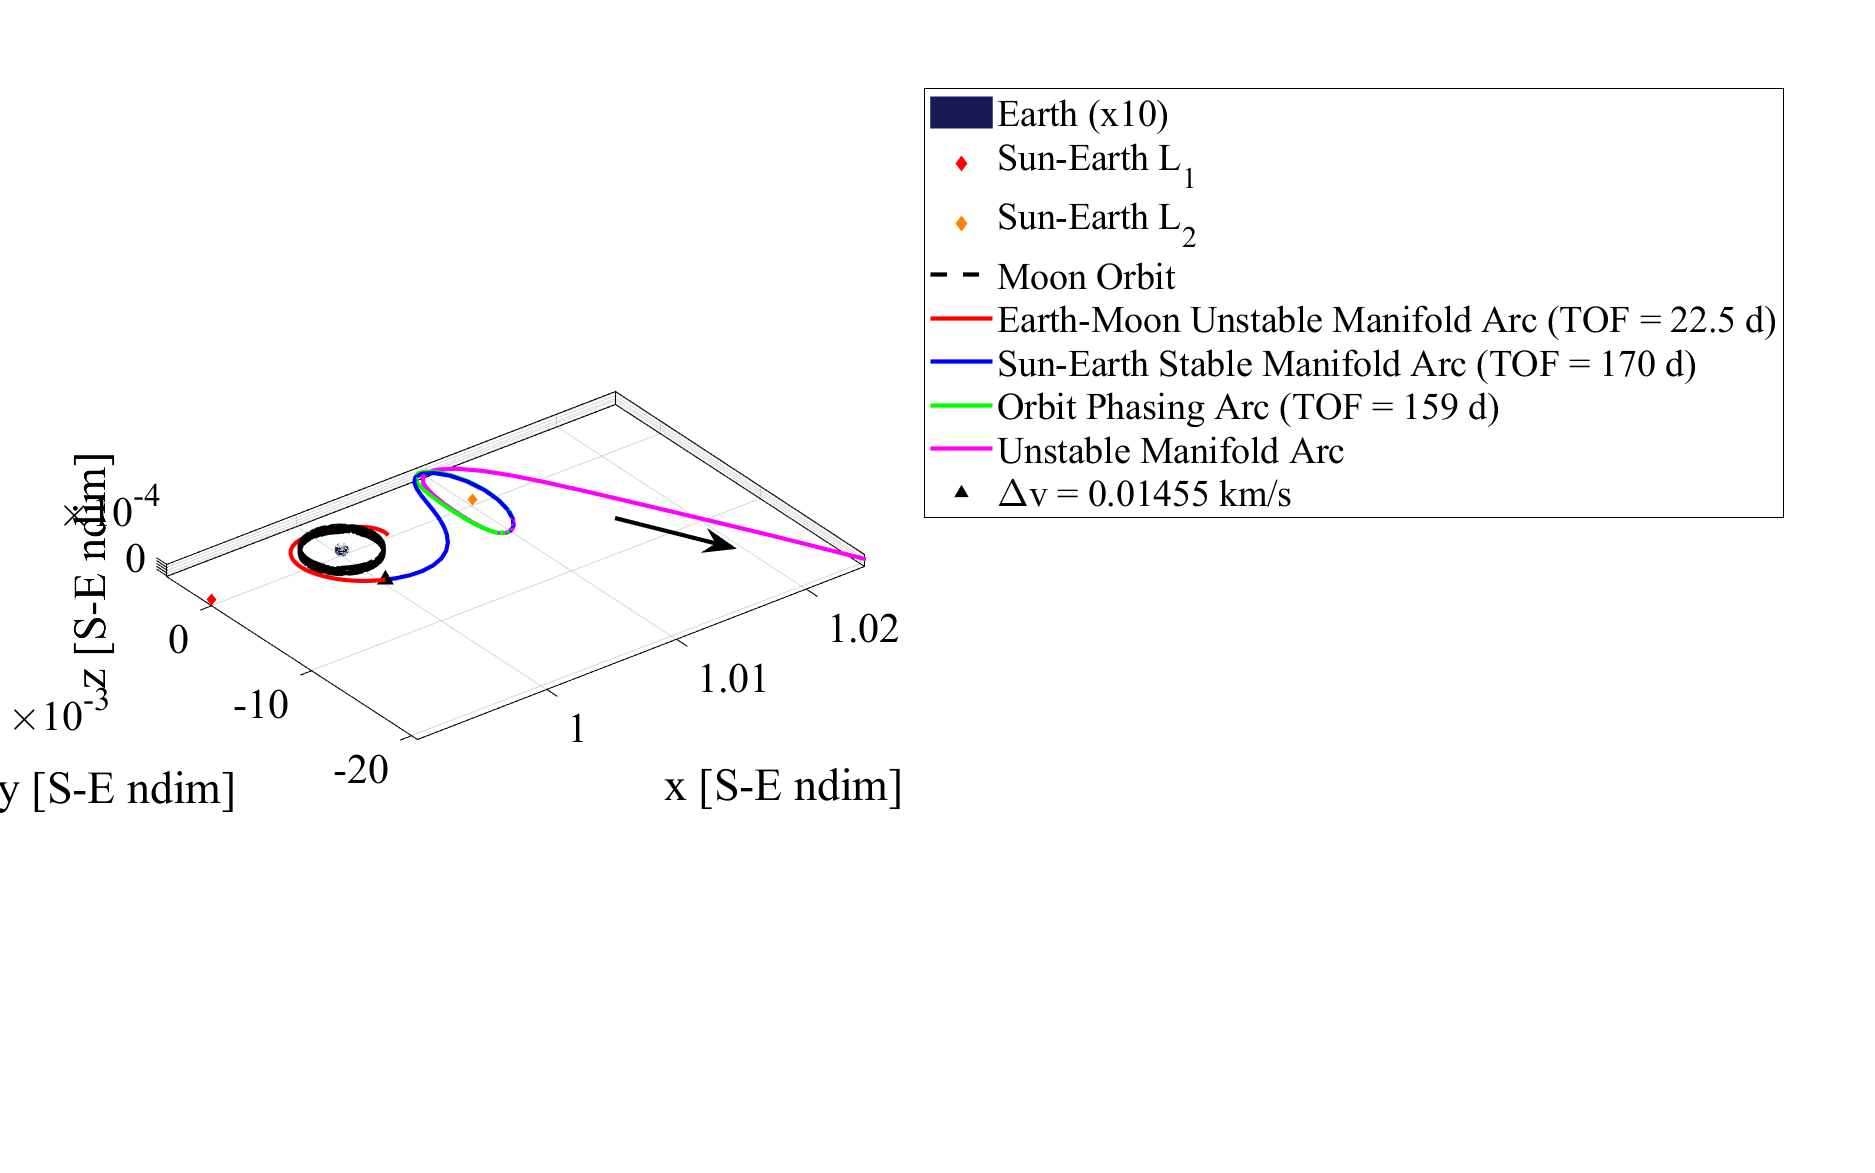
\includegraphics[width=0.9\textwidth]{figures/StagedMinTOFSE.pdf}
    \caption{Departure CR3BP arc with northern $L_{2}$ halo staging orbit ($JC=3.0008189$) in the Sun-Earth barycentric rotating frame for a low-TOF case.}
    \label{fig:stagedMinTOFSE}
\end{figure}

\begin{figure}[!htb]
    \centering
    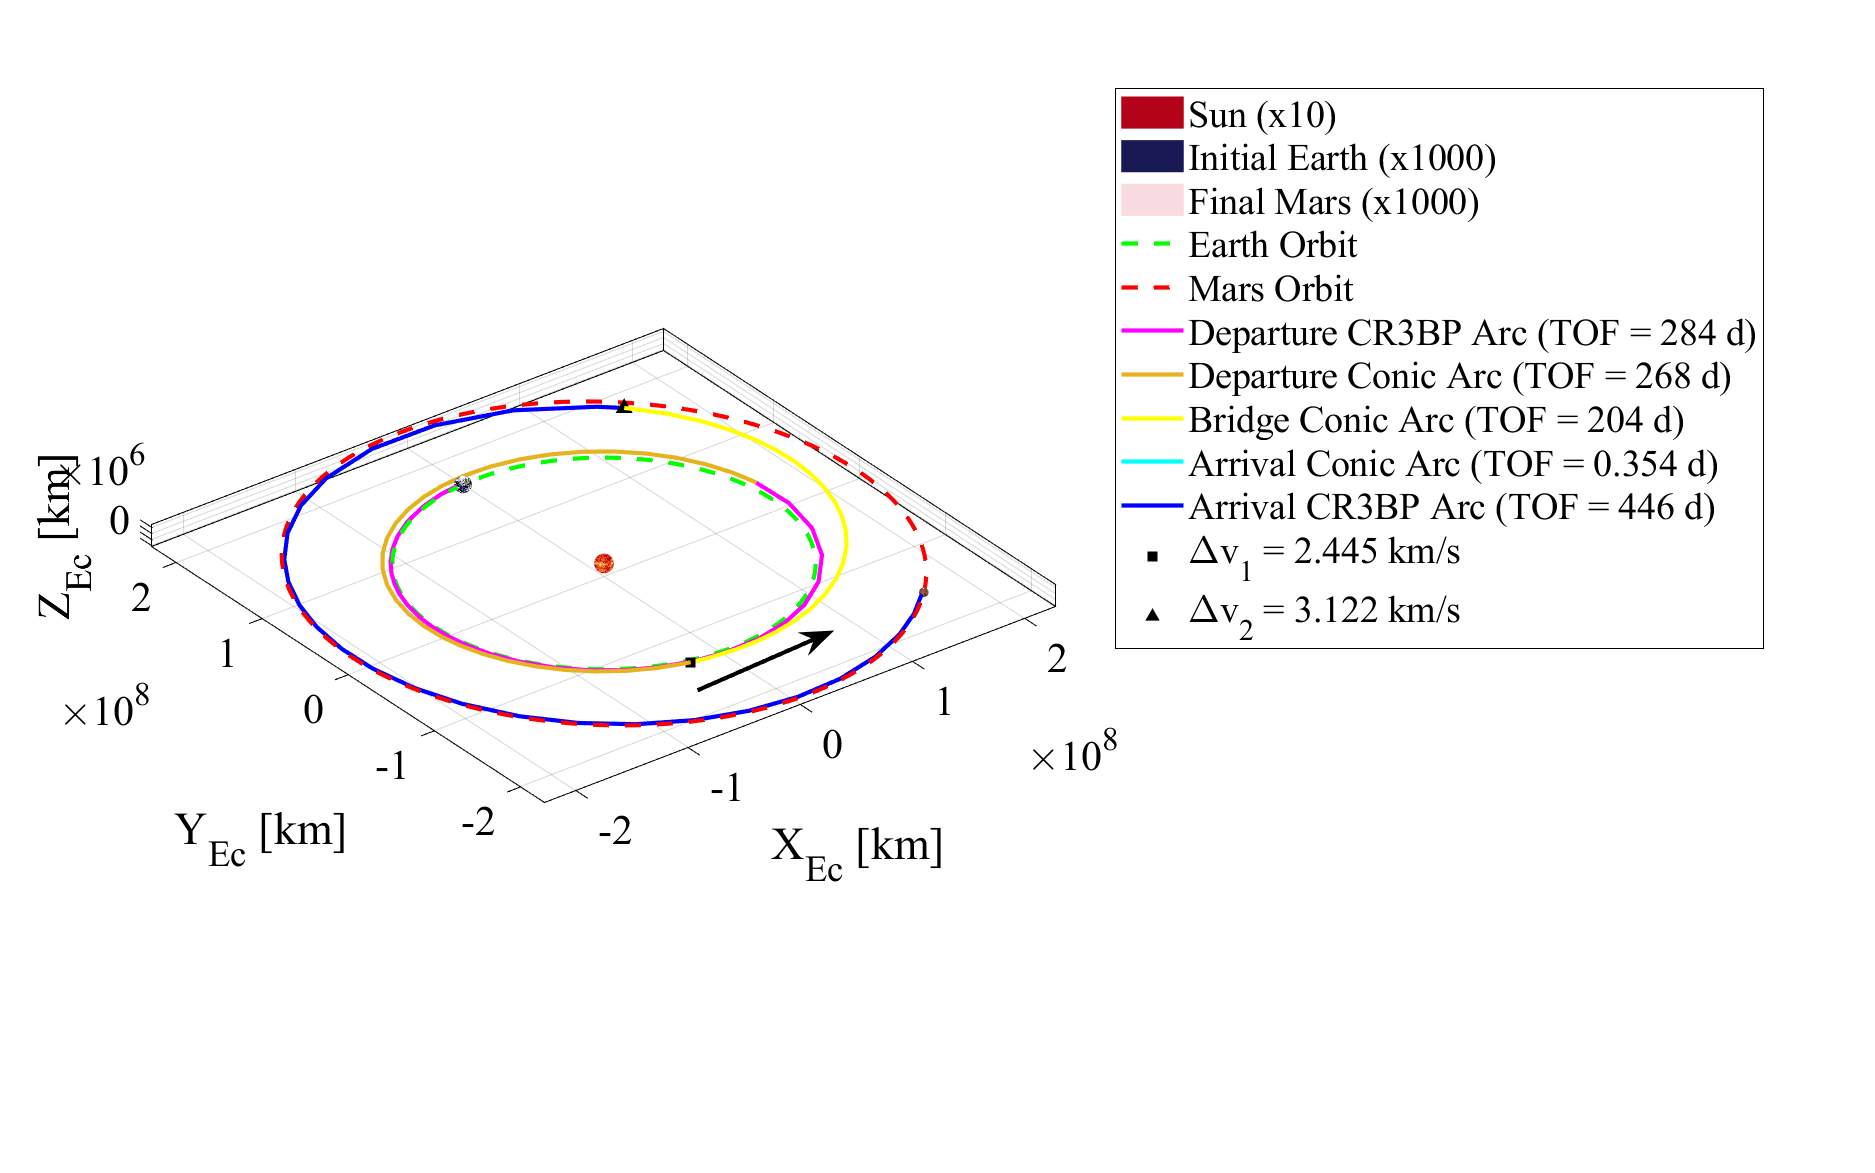
\includegraphics[width=0.9\textwidth]{figures/StagedMinTOFMMAT.pdf}
    \caption{MMAT in the Sun-centered Ecliptic J2000 frame for a staging orbit low-TOF case.}
    \label{fig:stagedMinTOFMMAT}
\end{figure}

\begin{figure}[!htb]
    \begin{subfigure}[h]{0.495\linewidth}
        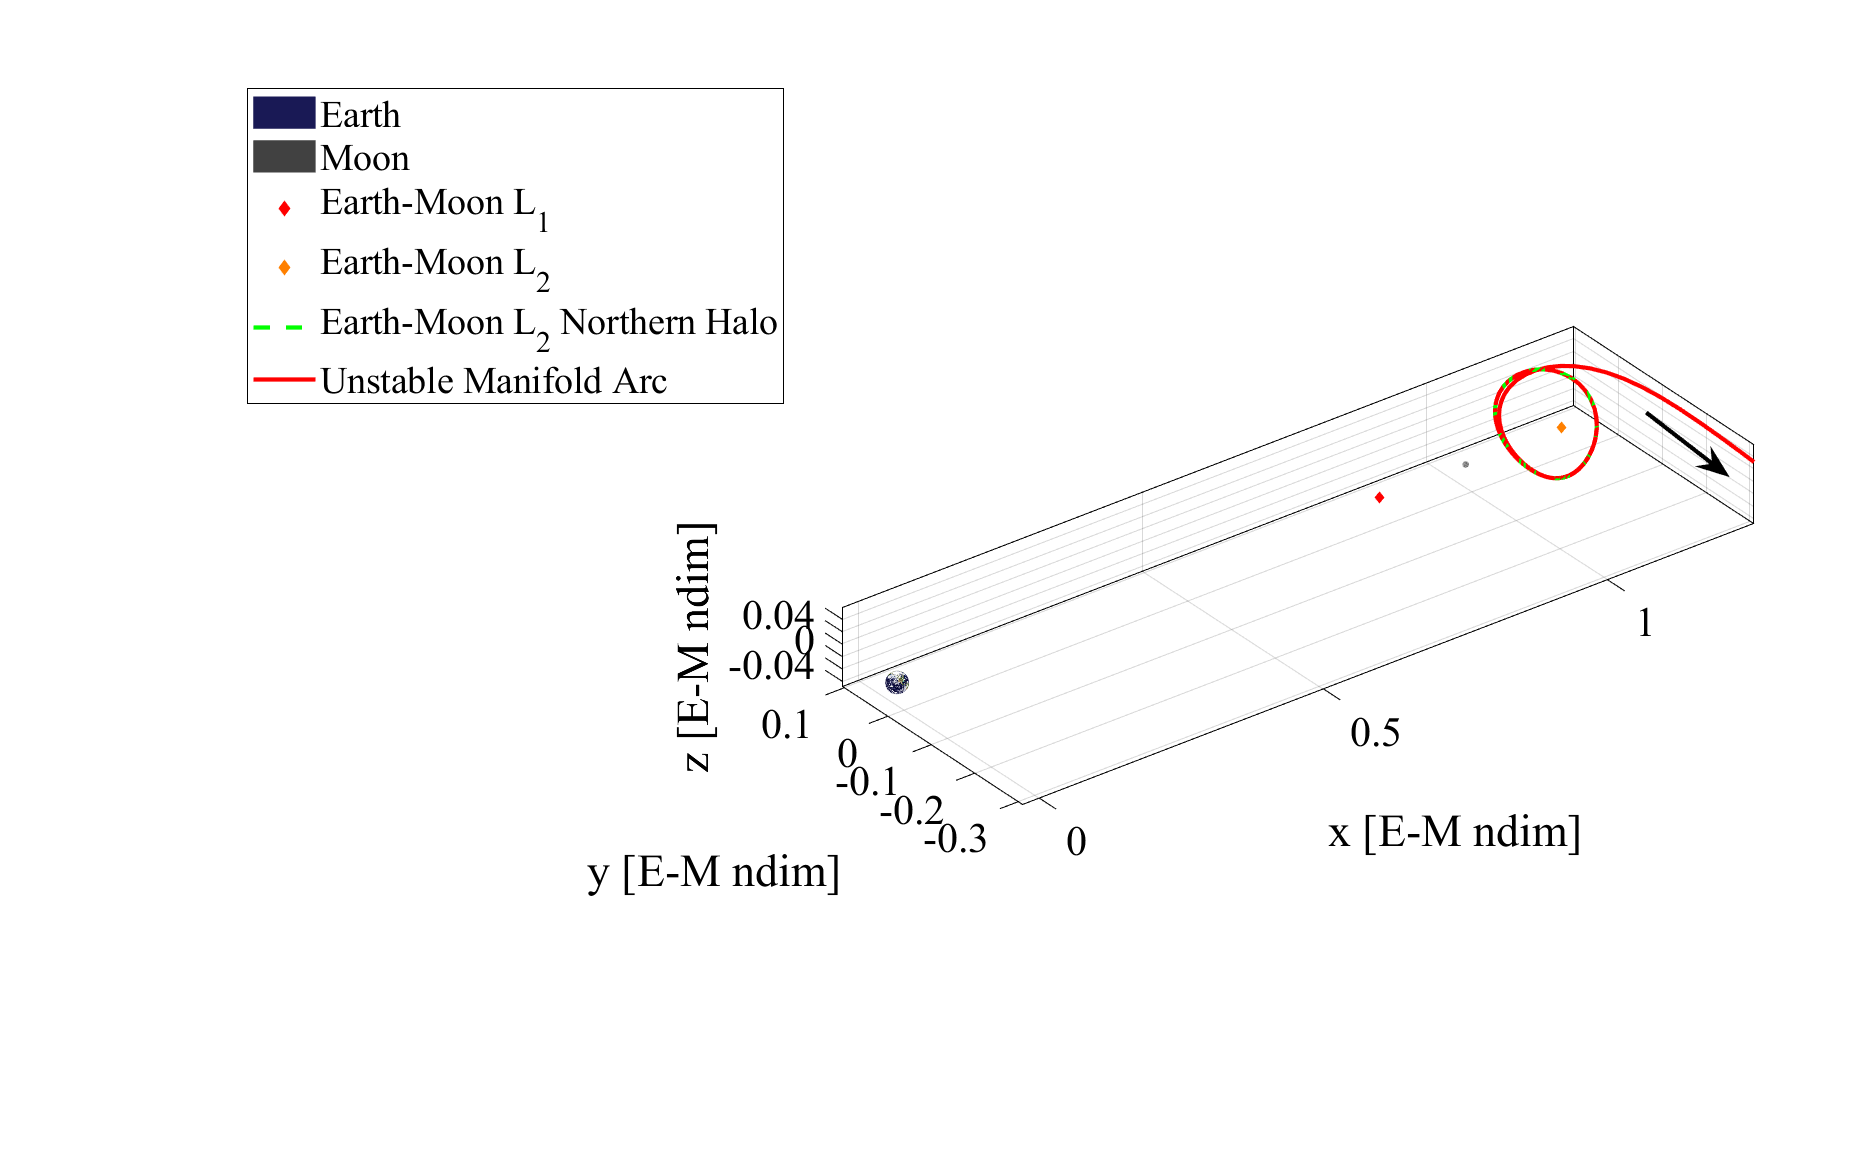
\includegraphics[width=\textwidth]{figures/DirectMinTOFEM.pdf}
        \caption{Earth-Moon barycentric rotating frame.}
    \end{subfigure}
    \hfill
    \begin{subfigure}[h]{0.495\linewidth}
        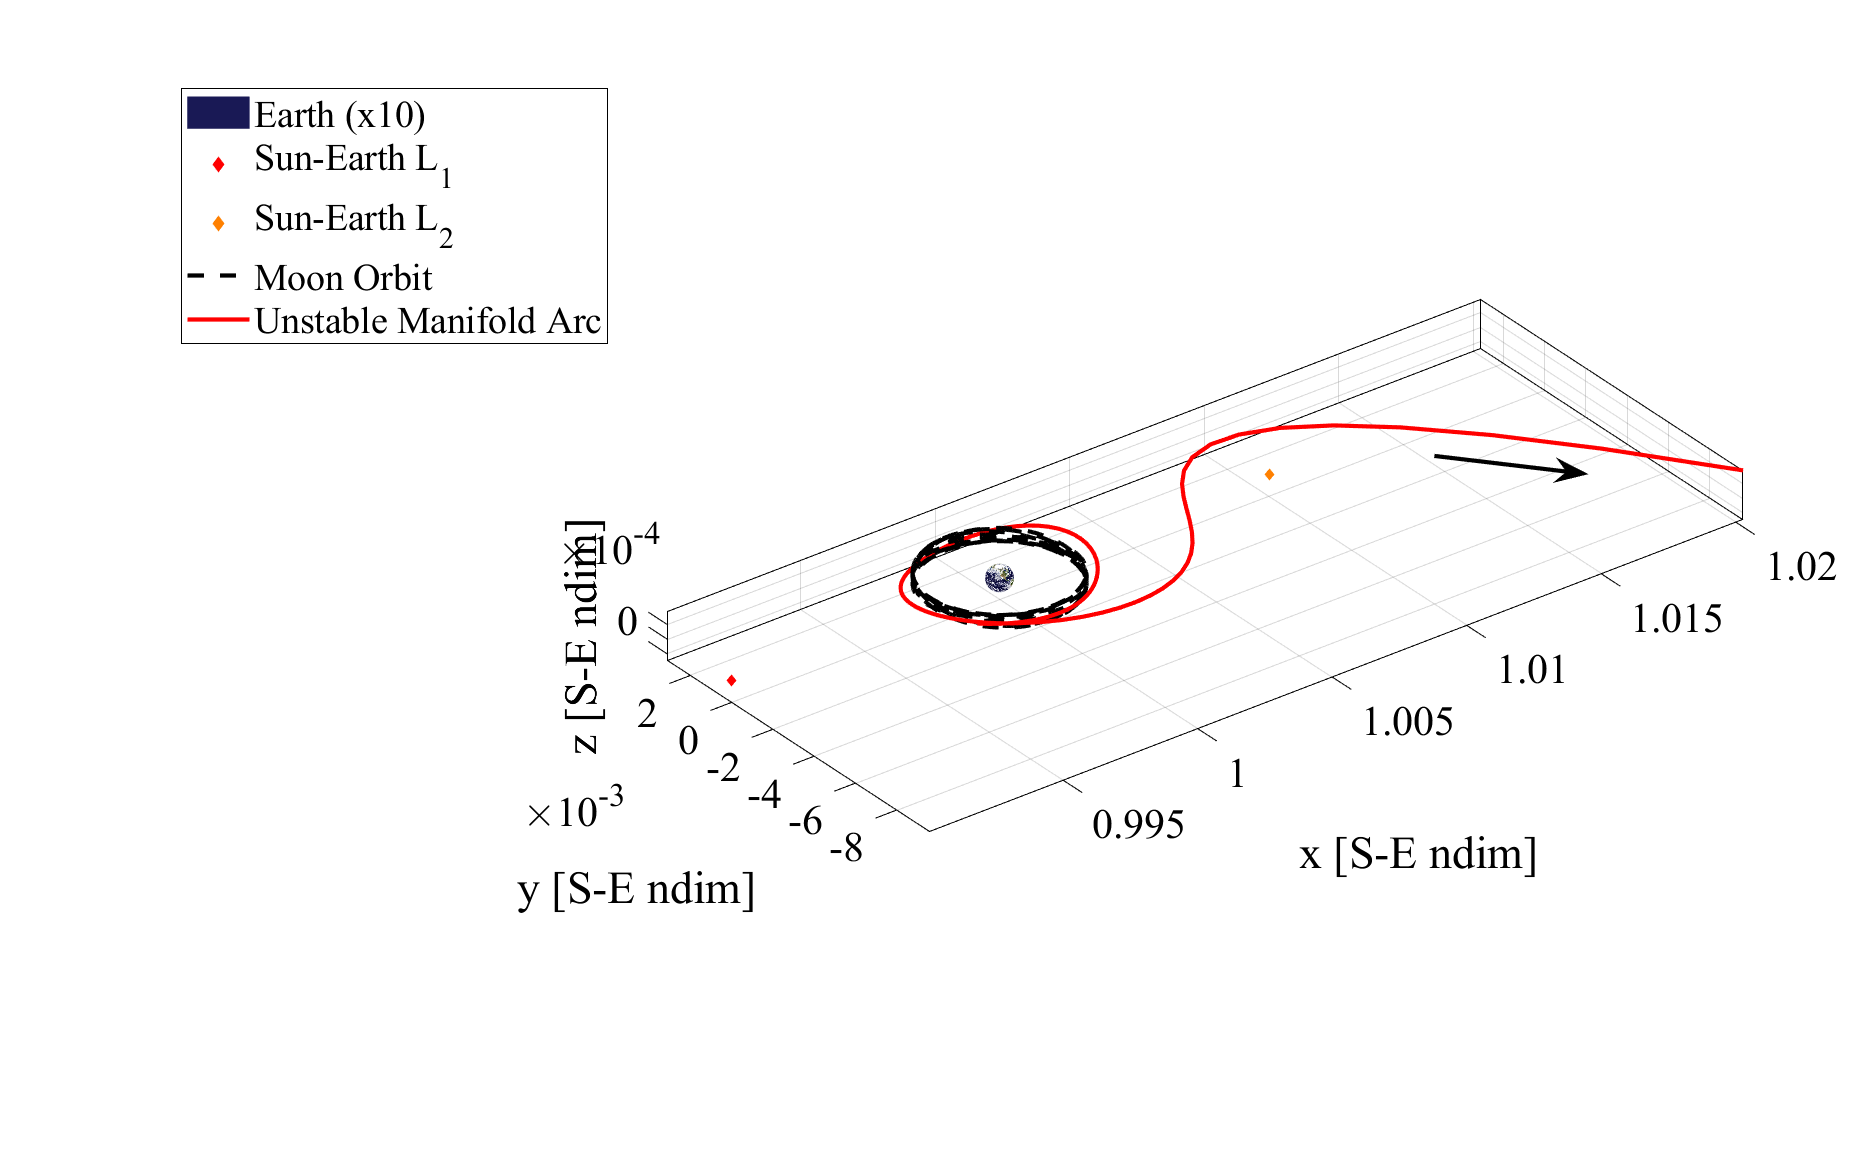
\includegraphics[width=\textwidth]{figures/DirectMinTOFSE.pdf}
        \caption{Sun-Earth barycentric rotating frame.}
    \end{subfigure}
    \caption{Northern $L_{2}$ halo orbit ($JC=3.13$) departure CR3BP arc for a low-TOF case.}
    \label{fig:directMinTOFE}
\end{figure}

\begin{figure}[!htb]
    \centering
    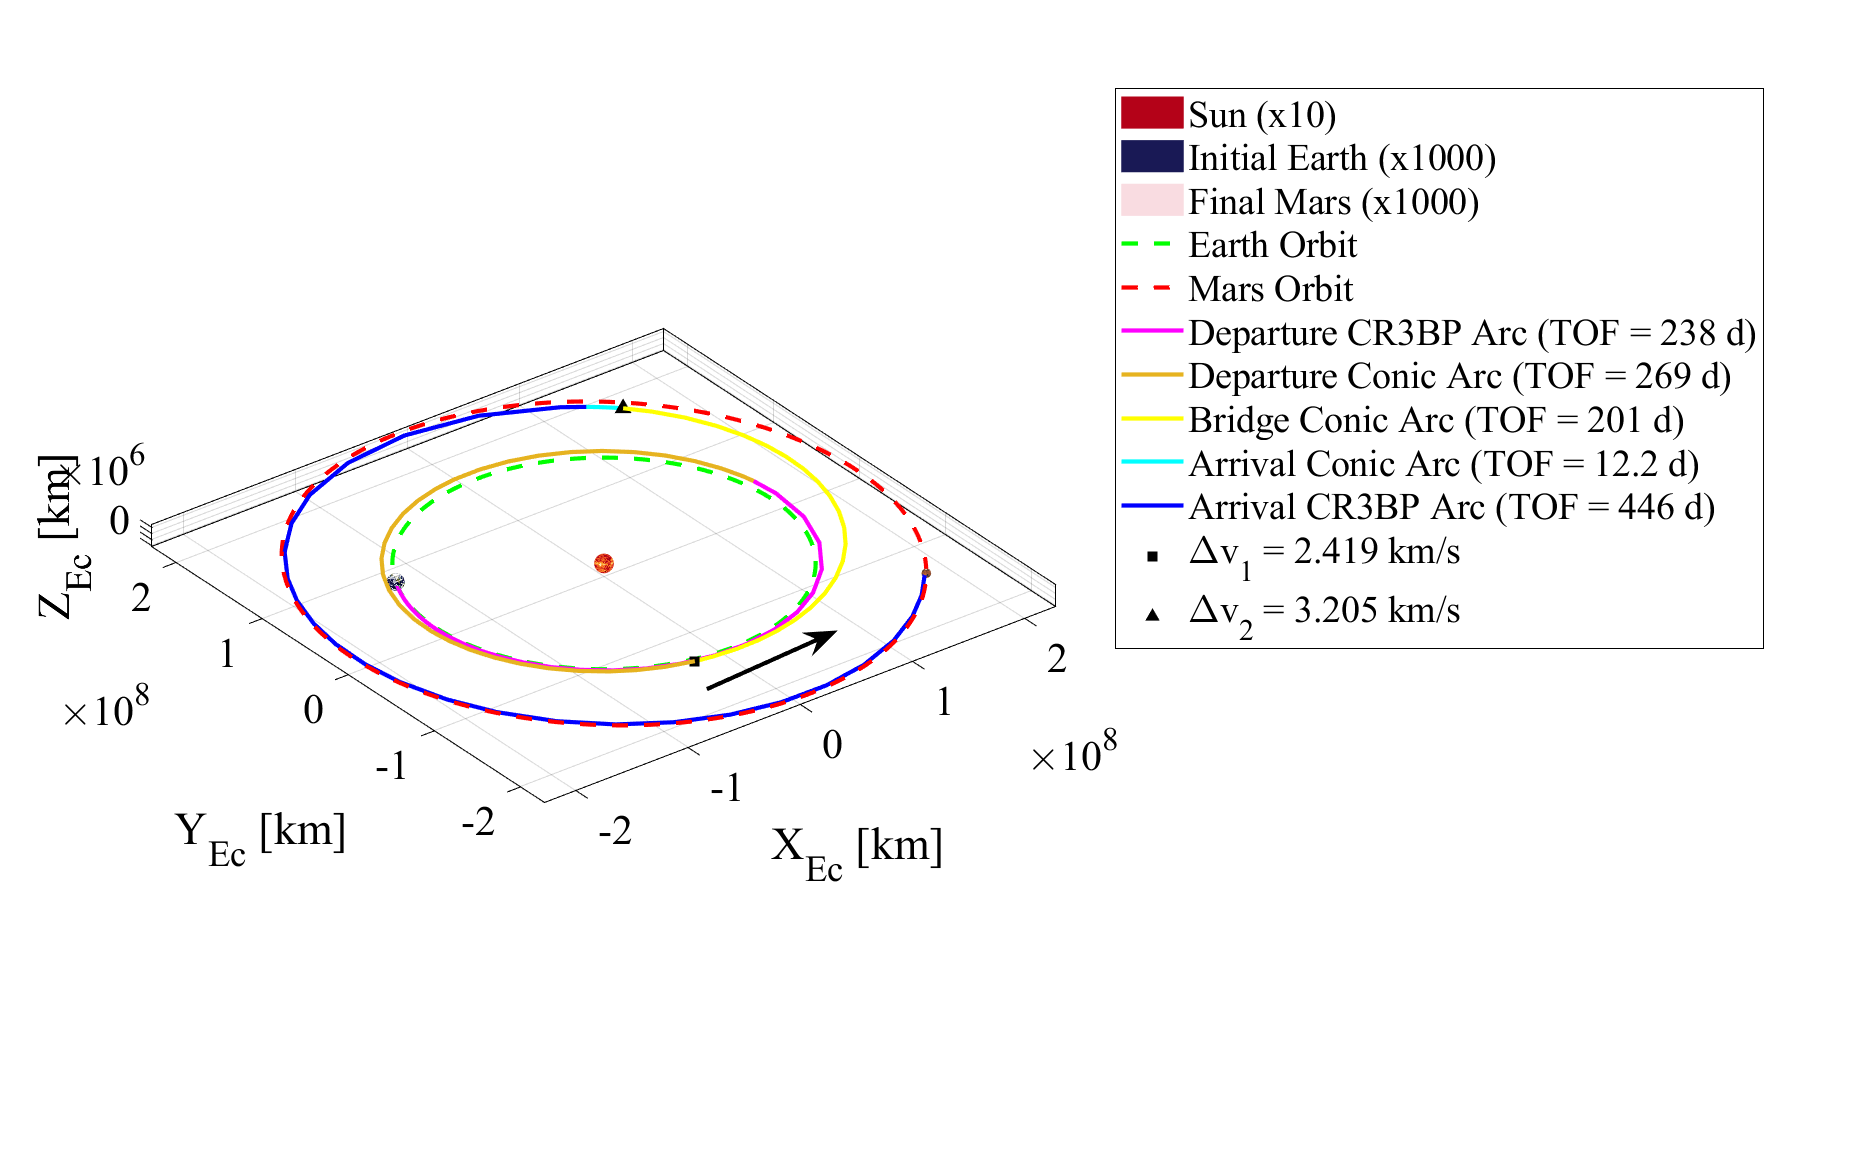
\includegraphics[width=0.9\textwidth]{figures/DirectMinTOFMMAT.pdf}
    \caption{MMAT in the Sun-centered Ecliptic J2000 frame for a direct low-TOF case.}
    \label{fig:directMinTOFMMAT}
\end{figure}

A few other ways to reduce the total transfer TOF involve the other three legs of the transfer.
Although the minimum-$\Delta v$ transfers occur when the bridge and arrival conic arc intersection
is $\ang{180}$ from the first MMAT maneuver, the bridge arc TOF can be decreased by moving the
final maneuver closer to the periapsis. While this will increase the maneuver cost, it can
sometimes be worth the flight time savings. Another option is to decrease the departure and arrival
CR3BP arc times-of-flight via the invariant manifold arc selections. Since some manifold arcs
depart faster from the system than others from the same orbit, this can lead to slight decreases in
TOF.

\subsection{Comparison between Departure Orbits}
Since both categories of transfers have similar average Maneuver $\Delta v$ costs among their best
solutions, it is easiest to evaluate the two types separately for that metric.
\cref{fig:compareDeltavStaged} compares the average best $\Delta v$ values for departures using
staging orbits from the orbits used in this investigation. As mentioned previously, no one orbit
family performs the best across the range of Jacobi constant values; however, some general trends
can be identified. Overall, these transfers perform better than the baseline modified Hohmann
transfer in terms of maneuver cost by around $0.5$ km/s while at each energy value, the spread
between the families is on the order of $0.2$ km/s. Some families show significant cost fluctuation
across energy levels while others do not. The families that seem to perform the best overall are
the $L_{1}$ halo and $L_{1}$ vertical families, although they are not necessarily the best choice
at each Jacobi constant. The $L_{2}$ axial family also performs well, but unfortunately, unstable
members only exist at lower Jacobi constant values. While it may not be the optimal choice in every
mission scenario, the lowest maneuver cost staging orbit transfers in this investigation originate
from the $3.03$ $L_{1}$ northern halo orbit, with an average total $\Delta v$ of $4.978$ km/s.
\cref{fig:stagedMinDvEM}-\cref{fig:stagedMinDvMMAT} show one such transfer from this specific
departure orbit.

\begin{figure}[!htb]
    \centering
    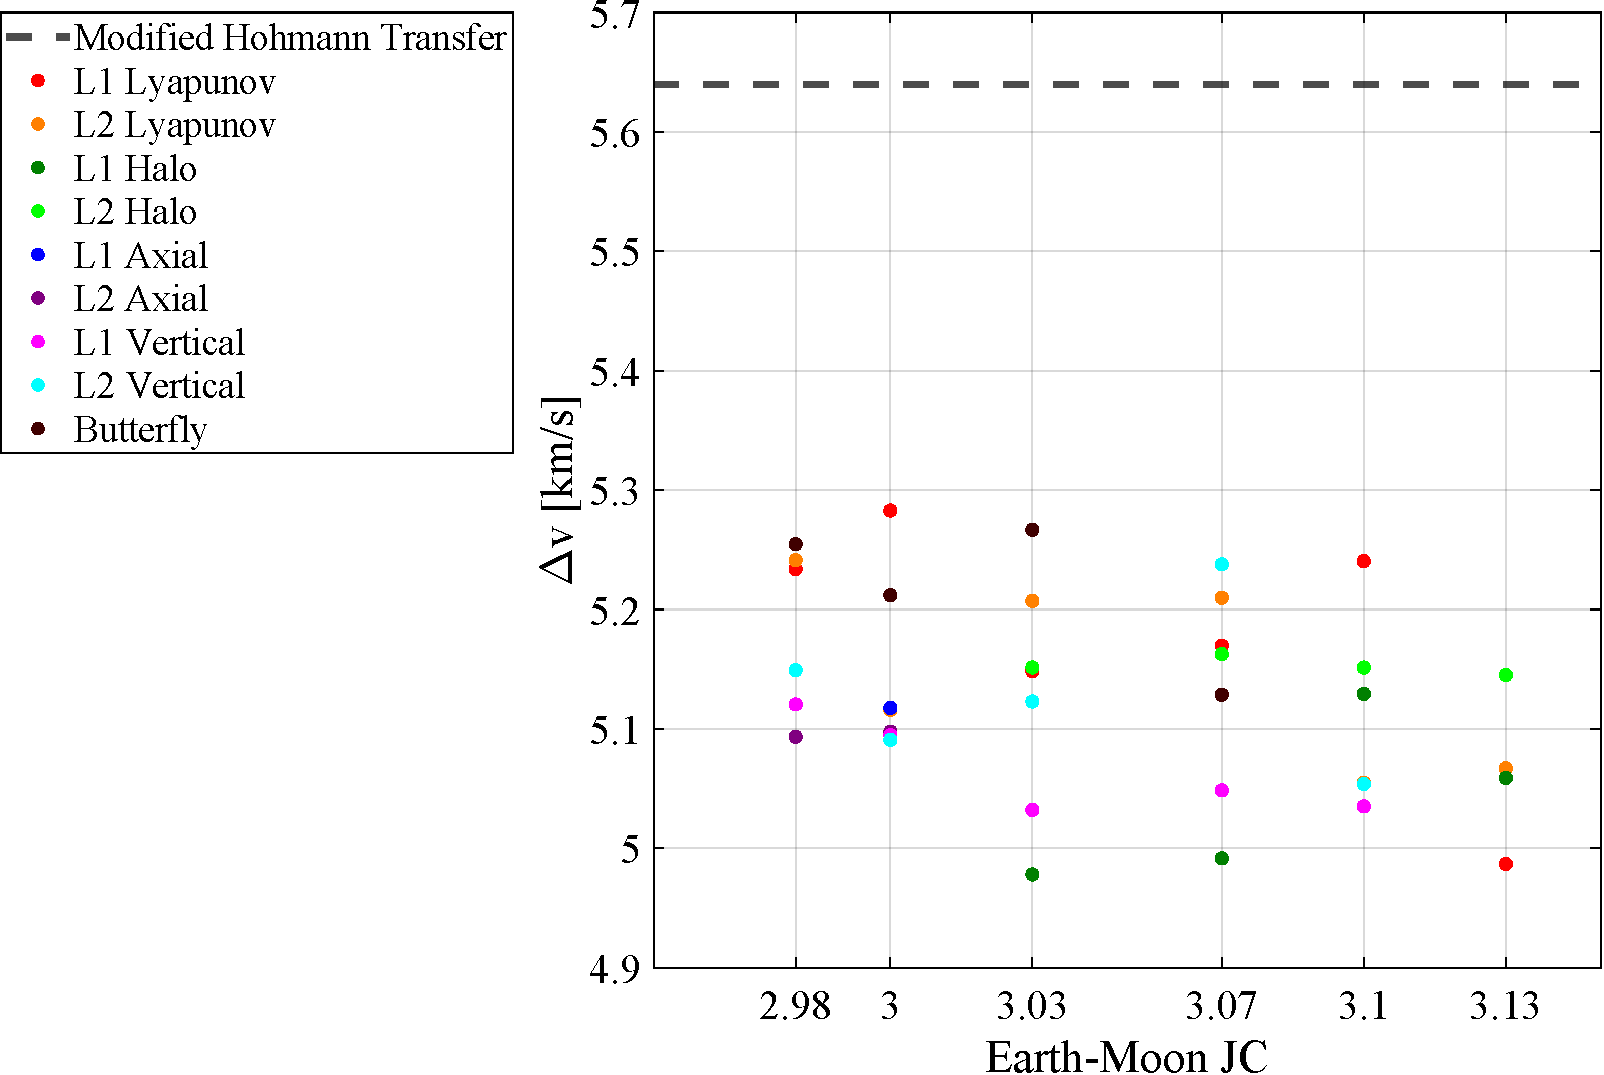
\includegraphics[width=0.9\textwidth]{figures/DeltavComparisonStaged.pdf}
    \caption{Average $\Delta v$ comparison between best transfers with staging orbits from various orbits/families.}
    \label{fig:compareDeltavStaged}
\end{figure}

Similarly, \cref{fig:compareDeltavDirect} shows the average best $\Delta v$ values for direct
departures. These orbits display similar performance on average to the staging orbit transfers in
comparison to the baseline modified Hohmann transfer. However, the lowest $\Delta v$ cases reach
nearly $0.8$ km/s improvement. The spread between the families is larger, reaching $0.5$ km/s for
some Jacobi values, but the variation across families is just as inconsistent as with the staging
orbit transfers. For these direct transfers, the $L_{1}$ Lyapunov orbit family performs the best by
far at every Jacobi constant value except $3.1$ (where it is one of the worst options). The $L_{1}$
halo family also performs well overall. The $3.0$ $L_{1}$ Lyapunov orbit provides the lowest
maneuver cost direct transfer with an average total $\Delta v$ of $4.791$ km/s. An example transfer
from this orbit is shown in \cref{fig:directMinDvE} and \cref{fig:directMinDvMMAT}.

\begin{figure}[!htb]
    \centering
    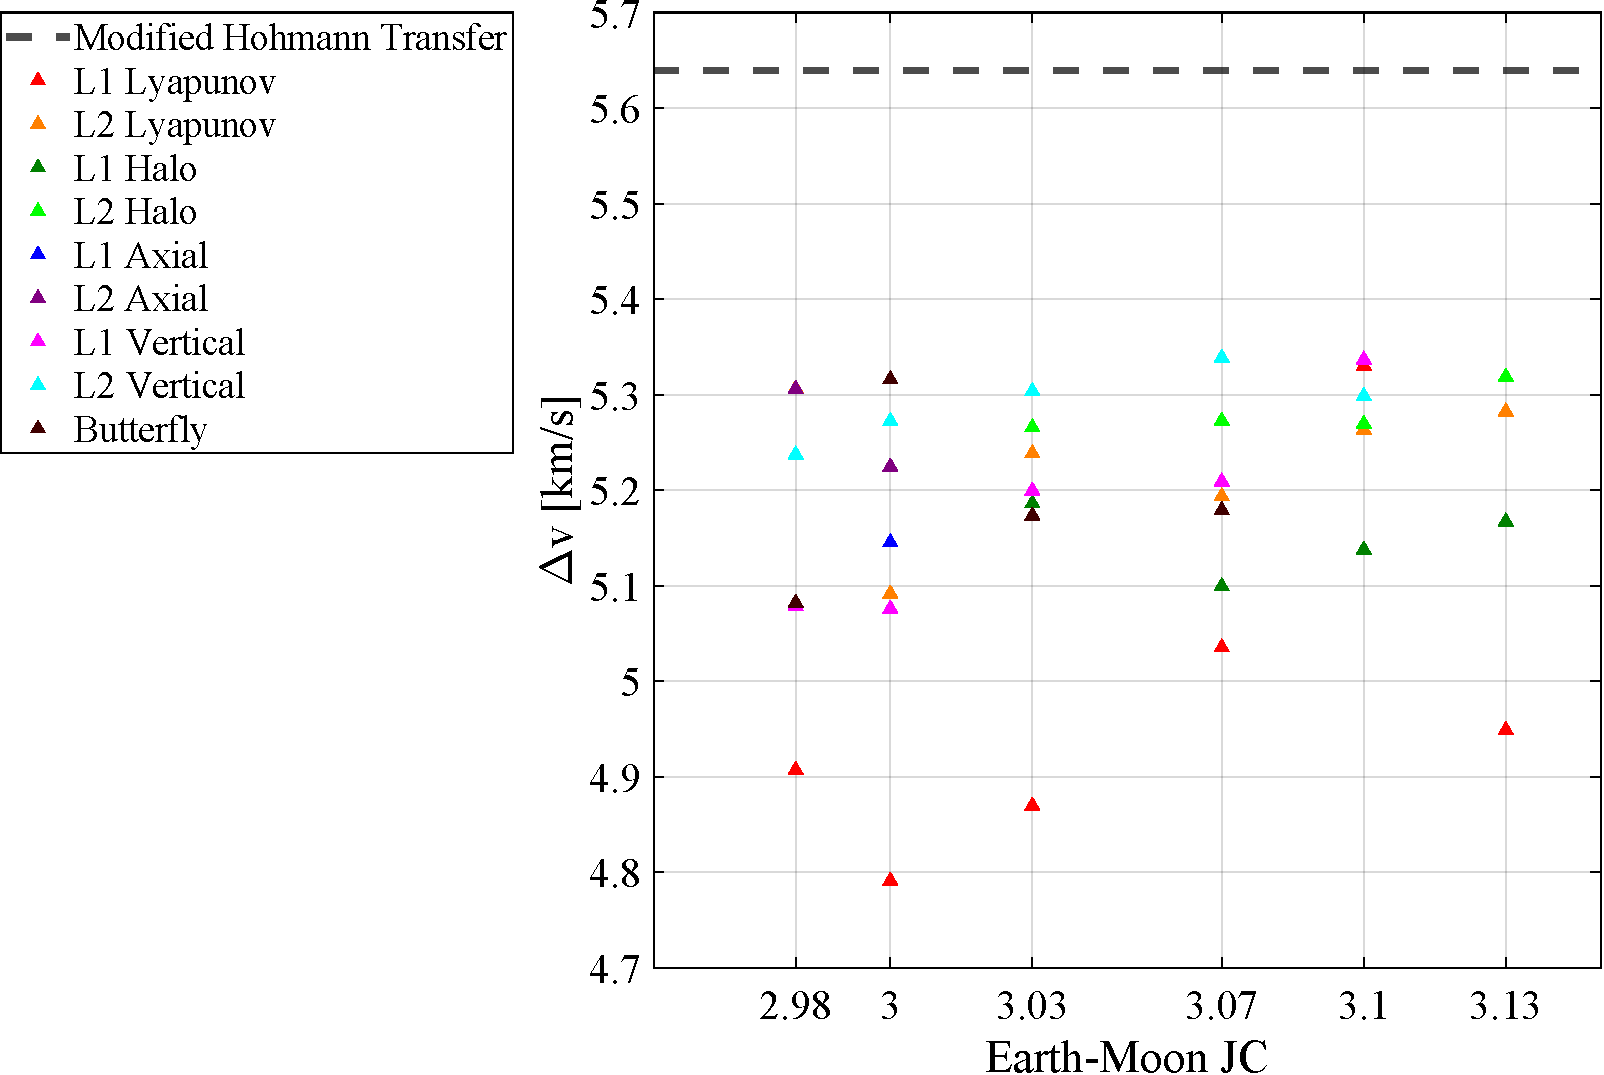
\includegraphics[width=0.9\textwidth]{figures/DeltavComparisonDirect.pdf}
    \caption{Average $\Delta v$ comparison between best transfers with direct departures from various orbits/families.}
    \label{fig:compareDeltavDirect}
\end{figure}

For both categories of transfers, $L_{1}$ orbit families seem to produce lower-$\Delta v$
transfers. It is likely that many of these transfers with invariant manifolds originating from
Earth-Moon $L_{1}$ departure families leverage close passes by the Moon to lessen the eventual
energy gap between the planetary systems, resulting in decreased maneuver costs. Again comparing
the two transfer types, in general, the best transfers with direct departures outperform the best
transfers with staging orbits in terms of maneuver costs. Nevertheless, both types see cost
reduction compared to the baseline modified Hohmann transfer.

When comparing the total transfer TOF between the two categories, the differences are large enough
to be evaluated directly in a single figure. \cref{fig:compareTOF} shows the average best TOF
values for both staging orbit transfers and those with direct departures. The staging orbit
transfers all lie in the range of $4.7$-$5.5$ years, while the direct transfer times-of-flight are
significantly lower in comparison: $3.9$-$4.6$ years. It is interesting to note that the energy
levels with higher times-of-flight for the staging orbit transfers are not the same as the higher
TOF options for direct transfers. The spread in TOF between the families at each Jacobi constant
value fluctuates both within each transfer type and overall. For instance, the $3.1$ direct
transfers have a spread of about $0.15$ years while it is $0.6$ at a Jacobi constant of $2.98$, and
the spread is near $0.3$ years for staged orbits at a Jacobi constant of $3.03$ but $0.6$ years for
$3.07$.

\begin{figure}[!htb]
    \centering
    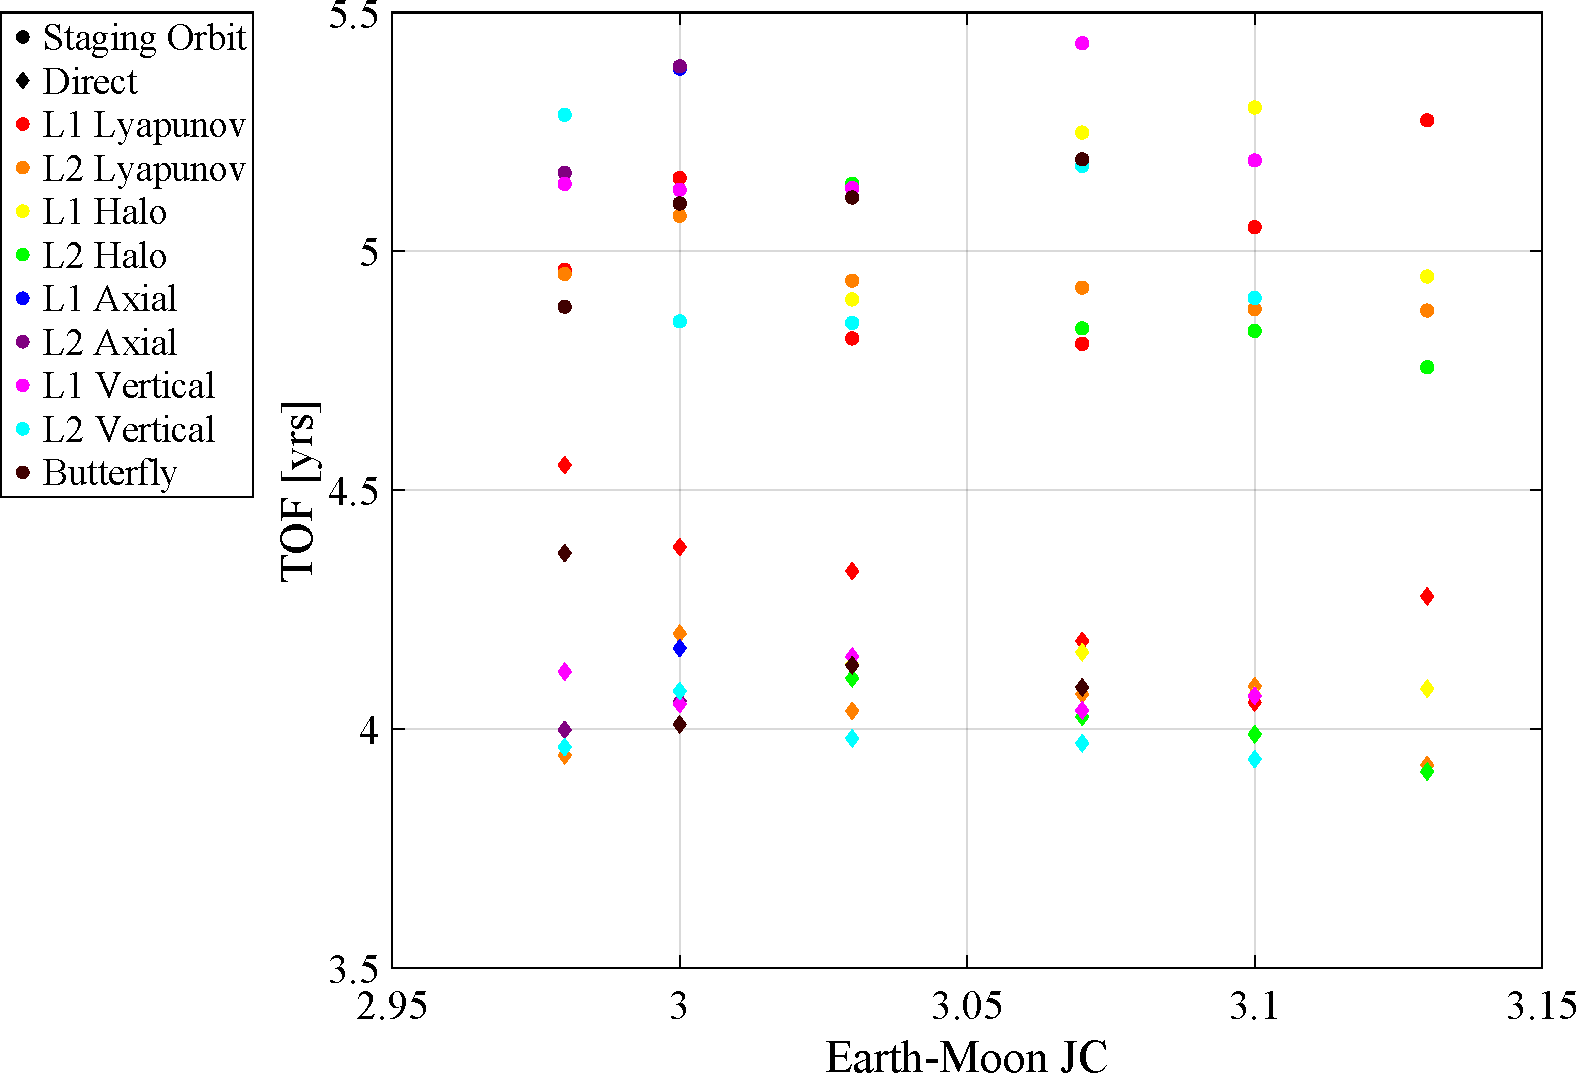
\includegraphics[width=0.9\textwidth]{figures/TOFComparison.pdf}
    \caption{Average TOF comparison between best transfers from various orbits/families.}
    \label{fig:compareTOF}
\end{figure}

Like with the total $\Delta v$ costs, the best total TOF values fluctuate unpredictably across each
family of orbits. Regardless, for the transfers with staging orbits, the $L_{2}$ Lyapunov and
$L_{2}$ halo orbits perform the best overall in TOF, although the results are a little less clear
than when comparing $\Delta v$ costs. The lowest TOF option investigated is the $3.13$ $L_{2}$
northern halo orbit, with an average total TOF of $4.76$ years, shown in
\cref{fig:stagedMinTOFEM}-\cref{fig:stagedMinTOFMMAT}. For the direct transfers, the $L_{2}$ halo
and $L_{2}$ butterfly orbits have the lowest times-of-flight. The $L_{2}$ axial orbits also perform
well at their limited energy values as before. In this category, the $3.13$ $L_{2}$ northern halo
orbit again performs the best with an average total TOF of $3.91$ years, shown in
\cref{fig:directMinDvE} and \cref{fig:directMinDvMMAT}. While $L_{1}$ departure orbits seem to
provide lower maneuver costs, \cref{fig:compareTOF} shows that $L_{2}$ departure orbits tend to
have lower best times-of-flight. This may be because the manifold arcs reach the Earth SoI faster
and extend slightly farther, decreasing the TOF of the transfer.

Many of the previous examples have shown that the transfers with lower total $\Delta v$ tend to
have higher times-of-flight and vice versa. Therefore, to find the departure orbits that provide
decreases in both, the best solutions are compared using $J$, the cost function value. The results
of this comparison are shown in \cref{fig:compareJ}. Immediately, it is clear once again that the
transfers with direct departures outperform those with staging orbits, with $J$ values near $31$
and $36$ respectively. Note that these $J$ values have little physical significance but are a
linear combination of the $\Delta v$ and TOF. The $J$ value spread at each Jacobi constant value is
similar to the spread in TOF in \cref{fig:compareTOF}.

\begin{figure}[!htb]
    \centering
    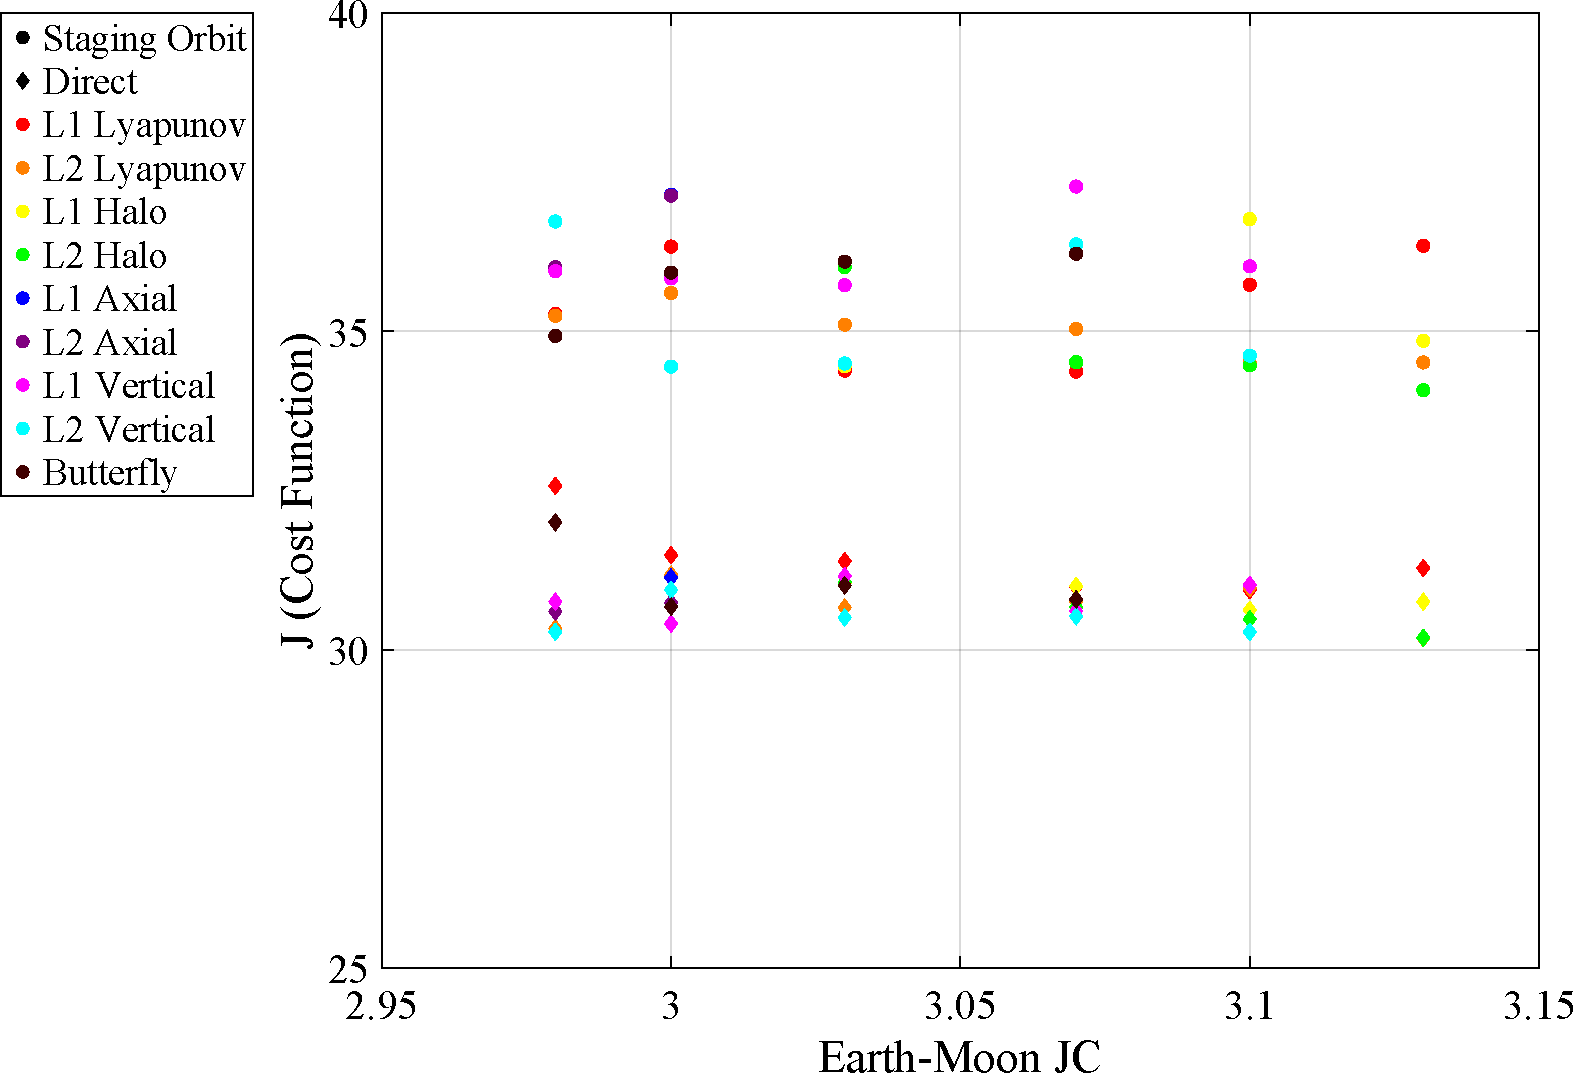
\includegraphics[width=0.9\textwidth]{figures/JComparison.pdf}
    \caption{Average cost function value comparison between best transfers from various orbits/families.}
    \label{fig:compareJ}
\end{figure}

In general, comparing the $J$ values between the departure orbits, it is less clear which families
perform the best. For the staging orbits, the $L_{2}$ halo orbits have lower costs at the higher
Jacobi constant values. At the lower Jacobi constants, the better families are different for each
case, although the $L_{2}$ Lyapunov orbits are consistently low throughout. Comparing the direct
transfers, the $L_{2}$ vertical orbit family performs well across the majority of the energy range,
with the $L_{2}$ halos again having low values at higher Jacobi constant orbits. The lowest overall
cost departure orbit is surprisingly the $3.13$ $L_{2}$ Lyapunov orbit direct departure, with an
average cost function value of $30.19$, an average total maneuver cost of $5.282$ km/s, and an
average total TOF of $3.92$ years. The best direct transfer from this departure orbit is shown
in \cref{fig:bestE} and \cref{fig:bestMMAT} with a total maneuver cost of $5.293$ km/s and TOF of
$3.24$ years.

\begin{figure}[!htb]
    \begin{subfigure}[h]{0.495\linewidth}
        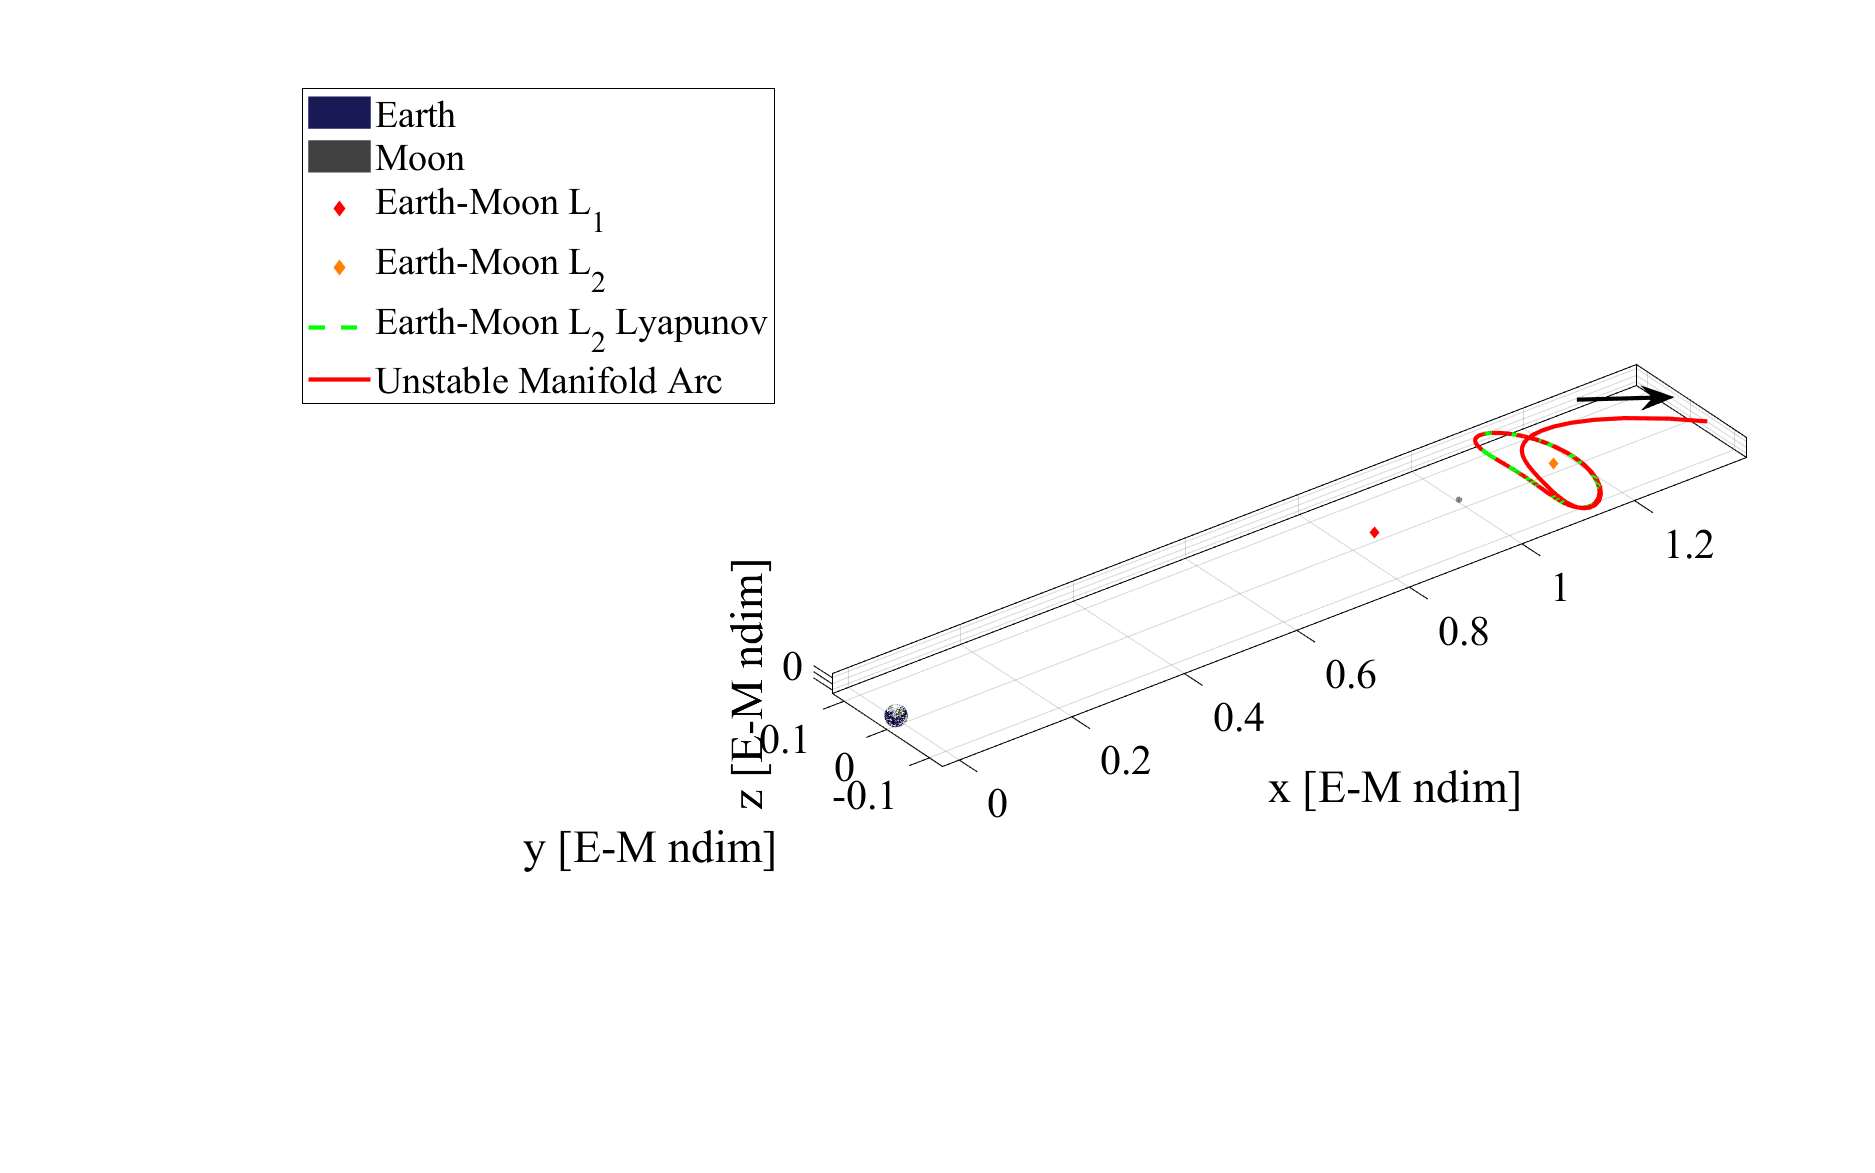
\includegraphics[width=\textwidth]{figures/BestEM.pdf}
        \caption{Earth-Moon barycentric rotating frame.}
    \end{subfigure}
    \hfill
    \begin{subfigure}[h]{0.495\linewidth}
        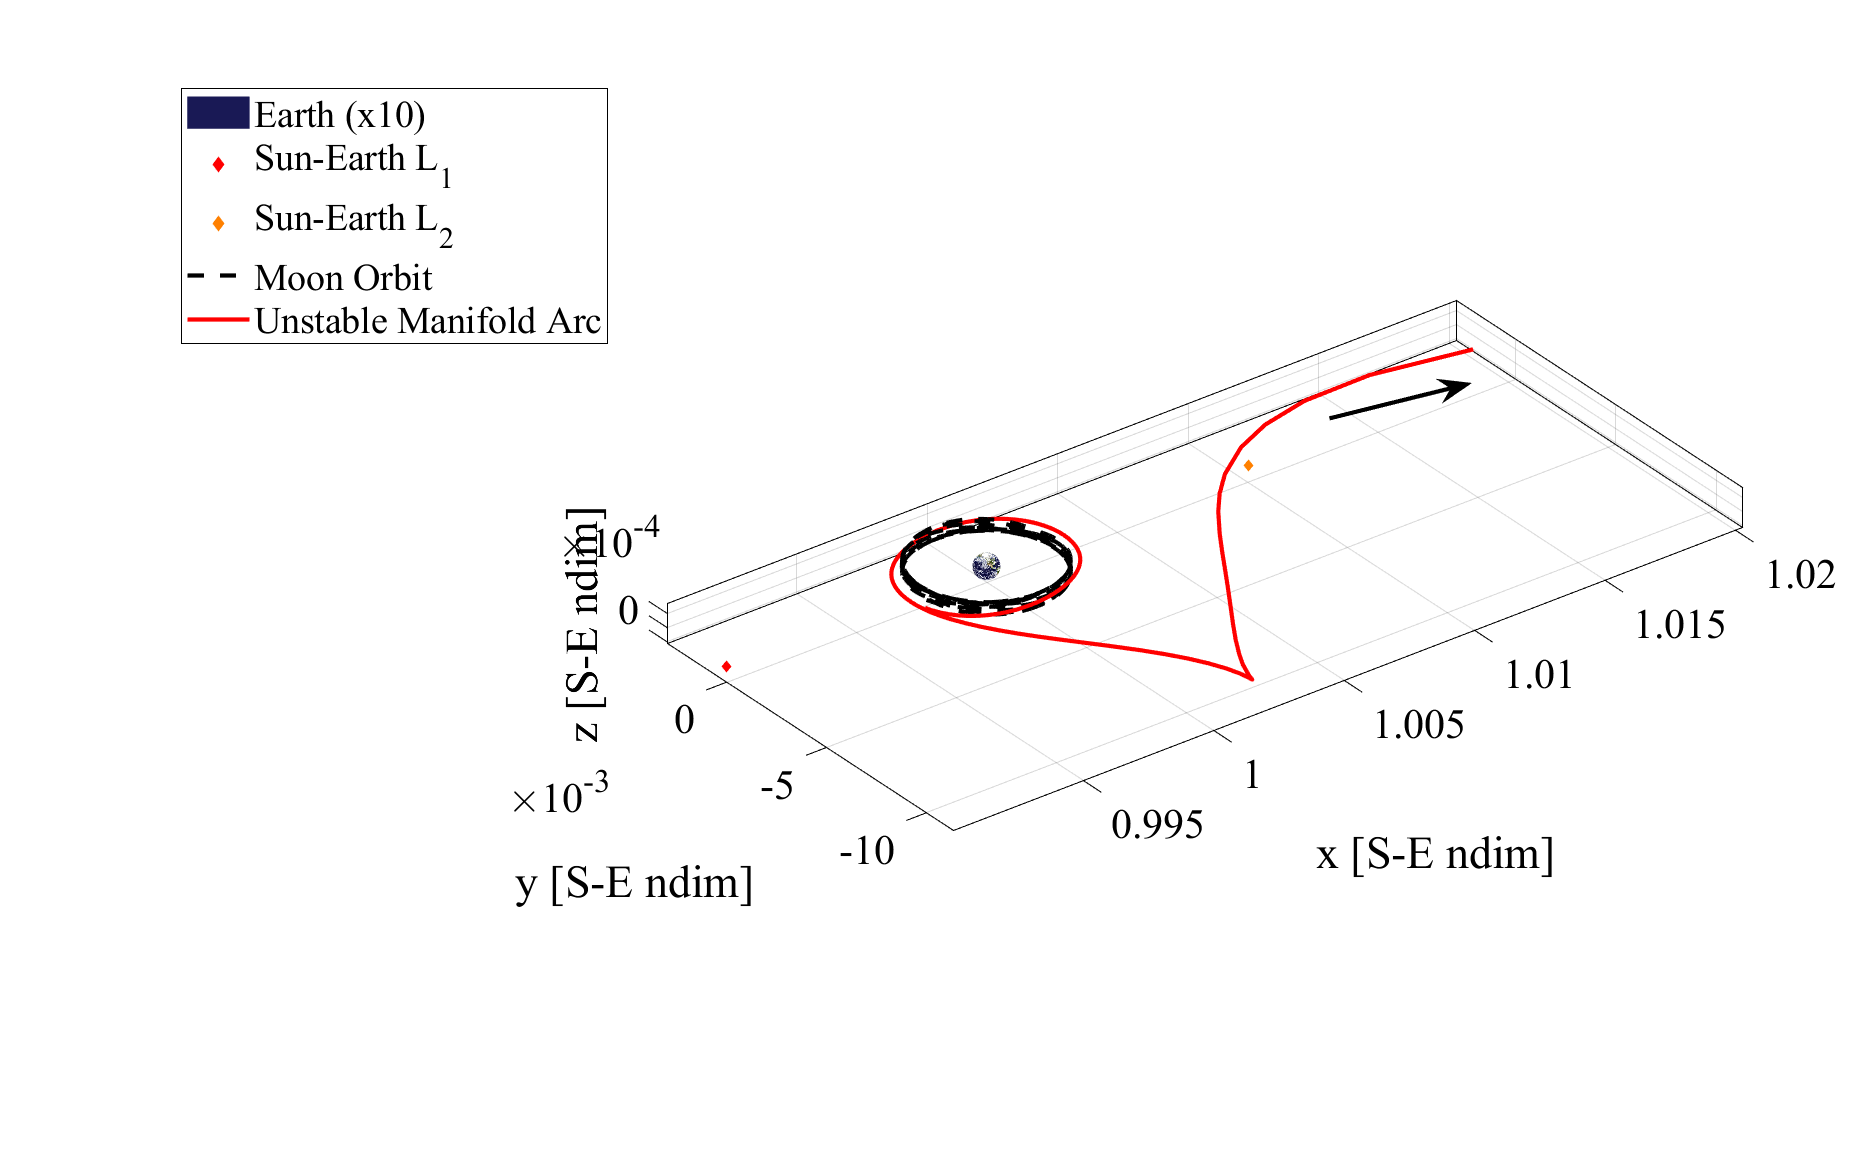
\includegraphics[width=\textwidth]{figures/BestSE.pdf}
        \caption{Sun-Earth barycentric rotating frame.}
    \end{subfigure}
    \caption{$L_{2}$ Lyapunov orbit ($JC=3.13$) departure CR3BP arc for best case.}
    \label{fig:bestE}
\end{figure}

\begin{figure}[!htb]
    \centering
    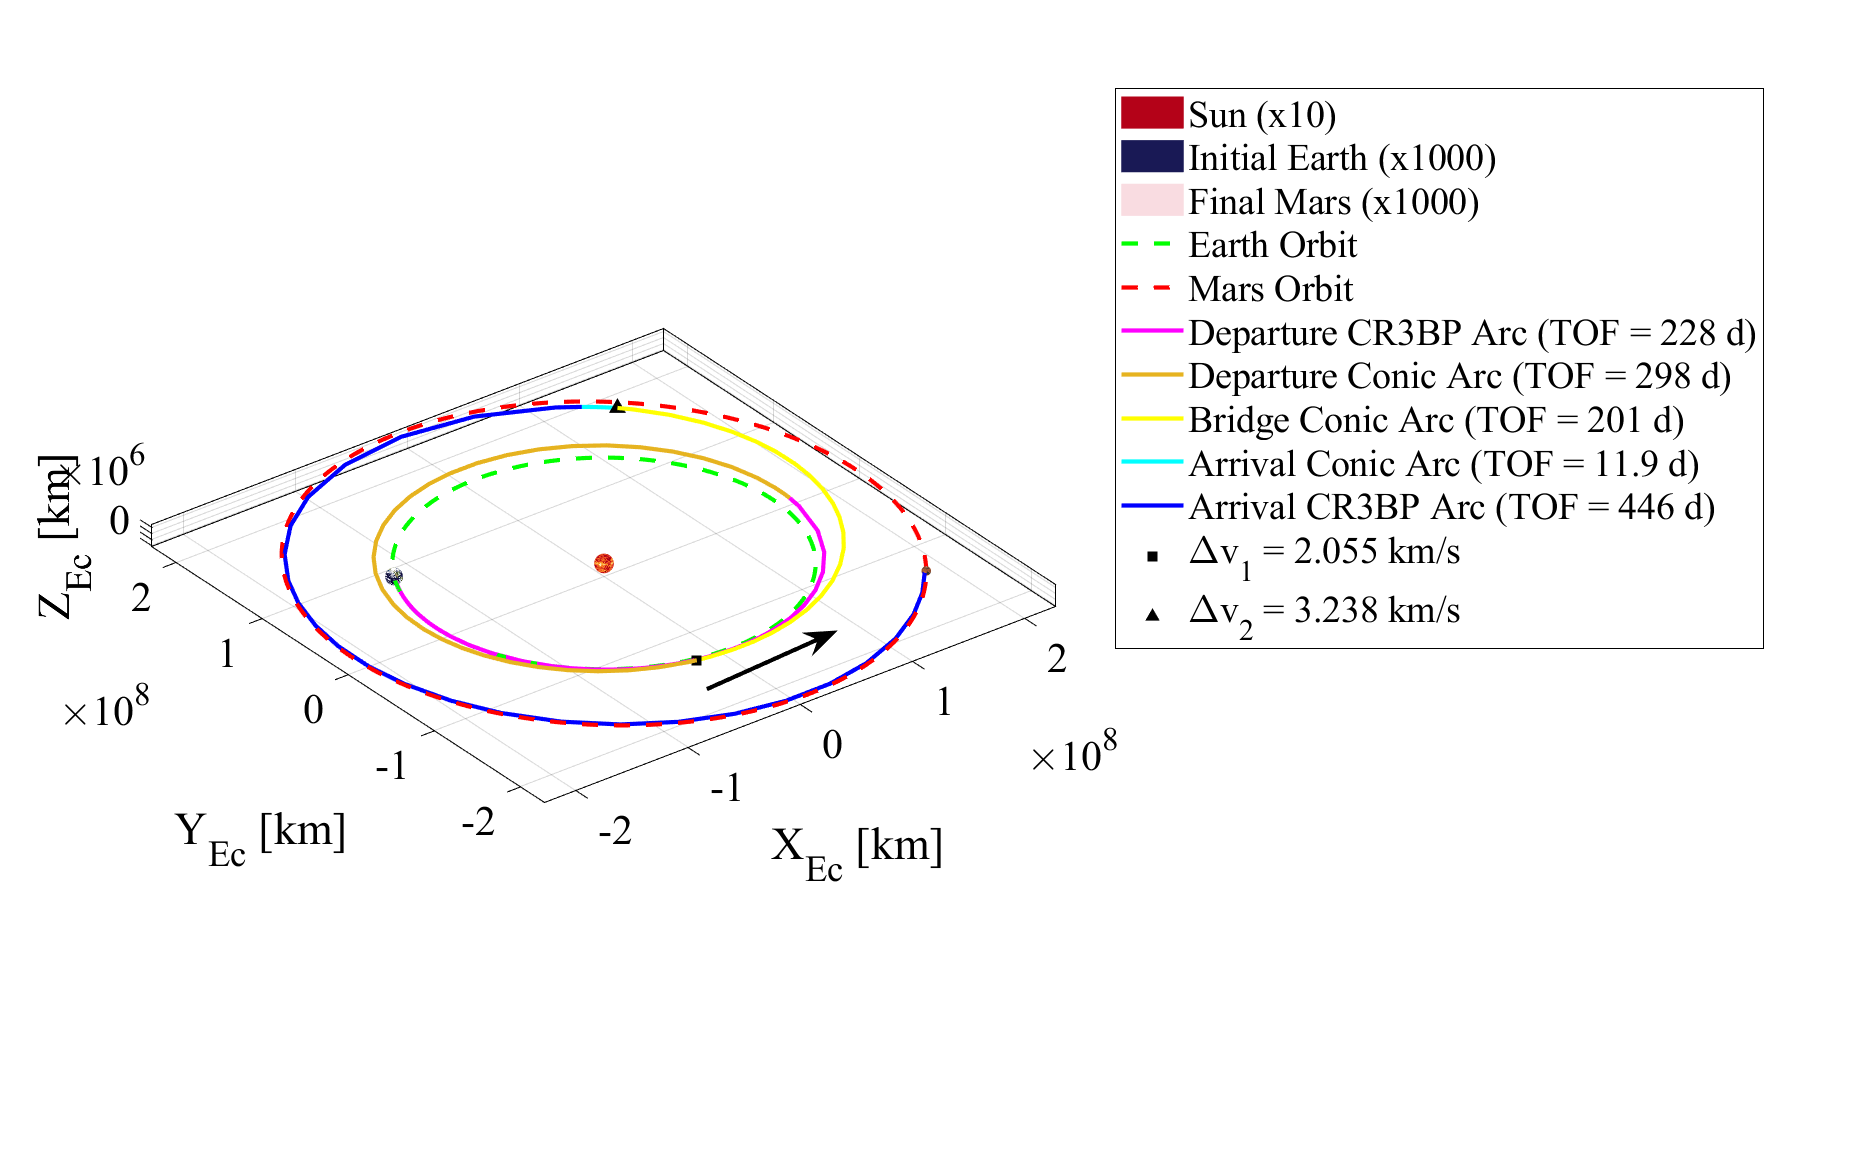
\includegraphics[width=0.9\textwidth]{figures/BestMMAT.pdf}
    \caption{MMAT in the Sun-centered Ecliptic J2000 frame for best case.}
    \label{fig:bestMMAT}
\end{figure}
